%\documentclass{book}\usepackage{sjtfonts}\usepackage{includegraphics}\usepackage{alltt}\usepackage{latexsym}
%\usepackage{array}
%\begin{document}\input{defs0}%		miradefs.tex 		    June 1994

% opening and closing a quoted Miranda section

\newcommand{\mira}{\noindent\hrulefill\nopagebreak\so}
\newcommand{\arim}{\nopagebreak\st\hrulefill\\}

% backslash in the Miranda environment
% Only feasible approach is to use \verb+\+
% in line!

%\newcommand{\bs}{$\mi\backslash\!\!$}
%\newcommand{\lbs}{\mbox{\verb+\+}}

% ignoring part of the input

\newcommand{\ignore}[1]{}

% a blank line in a Miranda section

\newcommand{\bl}{\mbox{\ }}

% Signalling a diffculty.

\definecolor{light-gray}{gray}{0.95}

\newcommand{\beware}[2]
 {\medskip\noindent\colorbox{light-gray}{\parbox{\textwidth}
 {\mbox{\large\textbf{#1}} \medskip\noindent\\ #2}\medskip\noindent}}

% Subscripting in Miranda text
\newcommand{\subscr}[2]{\mbox{${\mbox{\texttt{#1}}}_{\mbox{\texttt{#2}}}$}}

%\newcommand{\subscr}[2]{\mbox{${\mbox{\mi #1}}_{\mbox{\smtt #2}}$}}
\newcommand{\aone}{\subscr{a}{1}}
\newcommand{\atwo}{\subscr{a}{2}}
\newcommand{\ak}{\subscr{a}{k}}

\newcommand{\aoneone}{\subscr{a}{1,1}}

\newcommand{\eone}{\subscr{e}{1}}
\newcommand{\etwo}{\subscr{e}{2}}
\newcommand{\ei}{\subscr{e}{i}}
\newcommand{\er}{\subscr{e}{r}}

\newcommand{\fone}{\subscr{f}{1}}
\newcommand{\fl}{\subscr{f}{l}}

\newcommand{\gone}{\subscr{g}{1}}
\newcommand{\gtwo}{\subscr{g}{2}}
\newcommand{\gi}{\subscr{g}{i}}
\newcommand{\gr}{\subscr{g}{r}}

\newcommand{\hone}{\subscr{h}{1}}
\newcommand{\hl}{\subscr{h}{l}}

\newcommand{\pone}{\subscr{p}{1}}
\newcommand{\ptwo}{\subscr{p}{2}}
\newcommand{\pk}{\subscr{p}{k}}

\newcommand{\qone}{\subscr{q}{1}}
\newcommand{\qtwo}{\subscr{q}{2}}
\newcommand{\qk}{\subscr{q}{k}}

\newcommand{\rone}{\subscr{r}{1}}
\newcommand{\rtwo}{\subscr{r}{2}}

\newcommand{\tone}{\subscr{t}{1}}
\newcommand{\ttwo}{\subscr{t}{2}}
\newcommand{\tn}{\subscr{t}{n}}

\newcommand{\vone}{\subscr{v}{1}}
\newcommand{\vtwo}{\subscr{v}{2}}
\newcommand{\vn}{\subscr{v}{n}}

% for regular expressions

\newcommand{\stone}{\subscr{st}{1}}
\newcommand{\sttwo}{\subscr{st}{2}}
\newcommand{\stn}{\subscr{st}{n}}
\newcommand{\rthree}{\subscr{r}{3}}

\newcommand{\eps}{$\varepsilon$}
\newcommand{\trans}[1]{\stackrel{\mbox{\tt #1}}{\longrightarrow}}



% superscript in Miranda text

\newcommand{\superscr}[2]{\mbox{${\mbox{\mi #1}}^{\mbox{\smtt #2}}$}}

% Not equals in Miranda text

\newcommand{\noteq}{\makebox[0pt][l]{=}/}
\newcommand{\overslash}{\makebox[0pt][l]{/}}

% Definitions in complexity chapter

\newfont{\oldSym}{cmsy10}
\newcommand{\Th}{\boldmath$\oldSym\Theta$}
\newcommand{\pow}[1]{\^{}#1}
\newcommand{\leqq}{$\leq$}
\newcommand{\geqq}{$\geq$}
\newcommand{\lll}{$\ll$}
\newcommand{\eqq}{$\equiv$}
\newcommand{\ltwo}{\subscr{log}{2}}

% Indexing

\newcommand{\minx}[1]{\index{#1@{\ttfamily{}#1}}}
\setcounter{chapter}{16}\setcounter{page}{323}

\chapter{Lazy programming}
\chapstart
\label{lazy}
\index{lazy evaluation|(}

In our calculations so far we have said that the order in which we make
evaluation steps will not affect the results produced -- it may only affect
whether the sequence leads to a result. This chapter describes precisely the
\emph{lazy evaluation} strategy which underlies Haskell. Lazy evaluation is
well named: a lazy evaluator will only evaluate an argument to a function if
that argument's value is needed to compute the overall result.
Moreover, if an argument is structured (a list or a tuple, for instance),
only those parts of the argument which are needed to make the computation continue will be evaluated; we'll look at how this works in practice in some examples.

Lazy evaluation has consequences for the style of programs we can write. 
Since an intermediate list
will only be generated on demand, using an intermediate list will not
necessarily be expensive computationally. We examine this in the context of a
series of examples, culminating in a case study of parsing. 

To build
parsers we construct a \emph{toolkit} of polymorphic, higher-order
functions which can be combined in a flexible and extensible way to make
language processors of all sorts. One of the distinctive features of a 
functional language is the collection of facilities it provides for defining libraries like this; we'll come back to this example when we discuss domain-specific languages in Chapter \ref{dsls}.

We also take the opportunity to extend the \emph{list comprehension}
notation. This does not allow us to write any new programs, but does
make a lot of list processing programs -- especially those which work by
generating and then testing possible solutions
-- easier to express and understand.

Another consequence of lazy evaluation is that it is
possible for the language to describe \emph{infinite} structures. These
would require an infinite amount of time to evaluate fully, but under lazy
evaluation, only parts of a data structure need to be examined.  Any recursive
type will contain infinite objects; we concentrate on lists here, as infinite
lists are
by far the  most widely used infinite structures.

After introducing a variety of examples, such as infinite lists of prime and
random numbers, we discuss the importance of infinite lists for \emph{program
design}, and see that programs manipulating infinite lists can be thought of
as processes consuming and creating `streams' of data. Based on this idea, we
explore how to complete the simulation case study.

The chapter concludes with an update on program \emph{verification} in the light of
lazy evaluation and the existence of infinite lists; this section can only
give a flavour of the area, but contains references to more detailed
presentations.

Sections \ref{lazyEval} and \ref{calcRules} are essential reading, but the sections that follow explore the impact of laziness on a number of things we have looked at already, including list comprehensions and the simulation case study, as well as examining design and verification questions.

\section{Lazy evaluation}
\label{lazyEval}

Central to evaluation in Haskell is function application. The basic idea
behind this is simple: to evaluate the function \texttt{f} applied to arguments
\texttt{\subscr{a}{1}},  \texttt{\subscr{a}{2}}, \ldots , \texttt{\subscr{a}{k}}, we
simply \textbf{substitute} \index{substitution}
the expressions \texttt{\subscr{a}{i}} for the
corresponding variables in the definition of the function. For instance, if
\begin{alltt}
f x y = x+y
\end{alltt}
then 
\begin{alltt}
f (9-3) (f 34 3)
\step (9-3)+(f 34 3)
\end{alltt}
since we replace \texttt{x}  by \texttt{(9-3)} and \texttt{y} by \texttt{(f 34 3)}.
The expressions \texttt{(f 34 3)} and \texttt{(9-3)} are not evaluated
before they are passed to the function. 

In this case, for evaluation to continue, we need
to evaluate the arguments to `\texttt{+}', giving  
\begin{alltt}
\step 6+(f 34 3)
\step 6+(34+3) 
\step 6+37 
\step 43
\end{alltt}
In this example, both of the arguments are evaluated eventually, but this is not
always the case. If we define
\begin{alltt}
g x y = x+12
\end{alltt}
then 
\begin{alltt}
g (9-3) (g 34 3)
\step (9-3)+12 
\step 6+12 
\step 18
\end{alltt}
Here \texttt{(9-3)} is substituted for \texttt{x}, but as \texttt{y} does not appear
on the right-hand side of the equation, the argument \texttt{(g 34 3)} will
not appear in the result, and so is not evaluated. Here we see the first
advantage of lazy evaluation: \emph{an argument which is not needed will not be
evaluated}. This example is rather too simple: why would we write the second
argument if its value is never needed? A rather more realistic example is
\begin{alltt}
switch :: Integer -> a -> a -> a
switch n x y
  | n>0         = x
  | otherwise   = y
\end{alltt}
If the integer \texttt{n} is positive, the result is the value of
\texttt{x}; otherwise it is the value of
\texttt{y}. Either of
the arguments \texttt{x} and \texttt{y} might be used, but in the first
case \texttt{y} is not evaluated and in the second \texttt{x} is not
evaluated.
A third example is
\begin{alltt}
h x y = x+x
\end{alltt}
so that
\begin{alltt}
h (9-3) (h 34 3)\hfill (h-eval)
\step (9-3)+(9-3) 
\end{alltt}
It appears here that we will have to evaluate the argument \texttt{(9-3)}
twice since it is duplicated on substitution.\index{substitution!duplication on}
Lazy evaluation ensures that
\emph{a duplicated argument is never evaluated more than once}. This can be
modelled in a calculation by doing the corresponding steps simultaneously,
thus
\begin{alltt}
h (9-3) 17
\step (9-3)+(9-3) 
\step 6+6
\step 12 
\end{alltt}
In the implementation, there is no duplicated evaluation because
calculations are made over \textbf{graphs} \index{calculation!over graphs}
rather than trees to represent the expressions being evaluated.
For instance,
instead of duplicating the argument, as in (a) below, the evaluation of 
\texttt{(h-eval)} will give a graph in which on both sides of the plus there is the
{\em same\/} expression. This is shown in (b).
\begin{center}
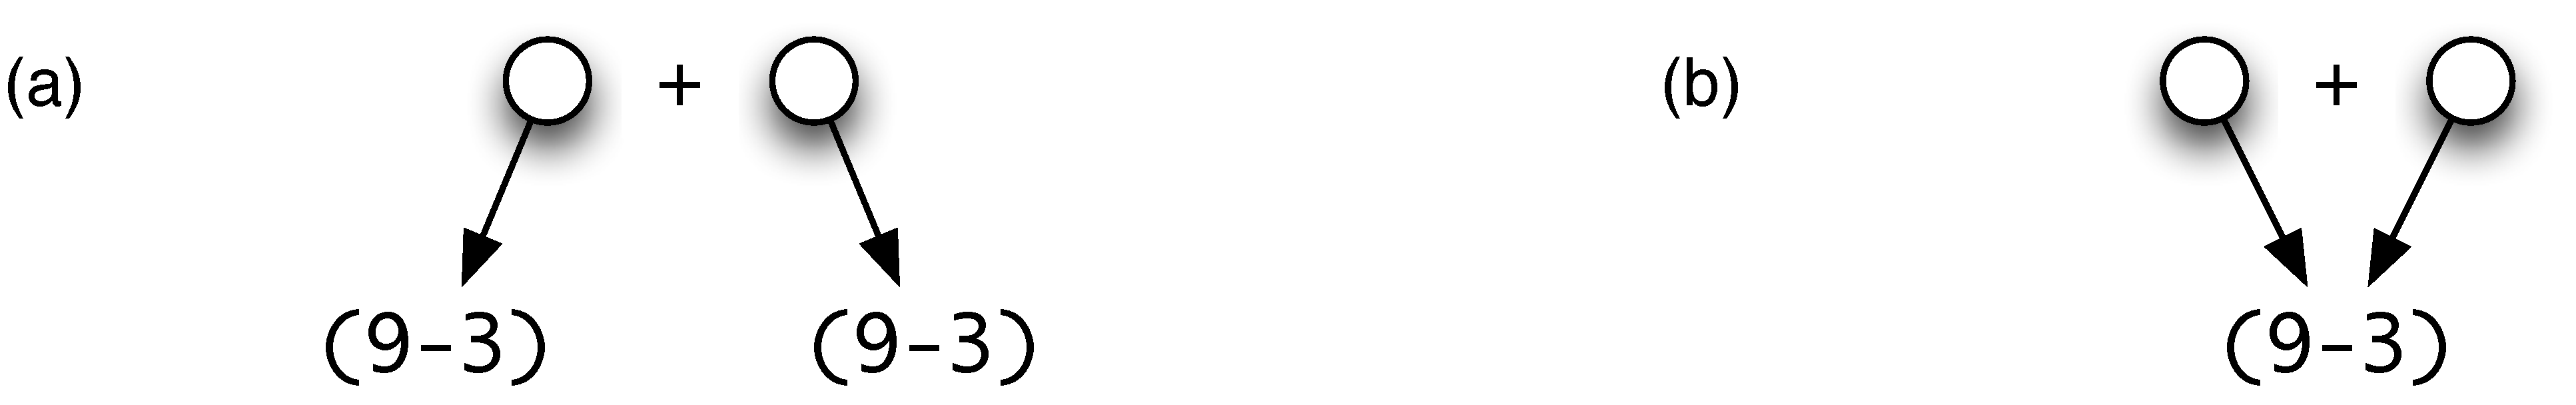
\includegraphics[width=4in]{Pictures/Sharing.pdf}
\end{center}
A final example is given by the pattern matching \index{pattern matching}
function,
\begin{alltt}
pm (x,y) = x+1
\end{alltt}
applied to the pair \texttt{(3+2,4-17)}. 
\begin{alltt}
pm (3+2,4-17)
\step (3+2)+1
\step 6
\end{alltt}
The argument is examined, and part of it is evaluated. The second
half of the pair remains unevaluated, as it is not needed in the calculation.
This completes the informal introduction to lazy evaluation, which can be
summarized in the three points:
\begin{titemize}
\item arguments to functions are evaluated only when this is necessary for
evaluation to continue;
\item an argument is not necessarily evaluated fully: only the parts that are
needed are examined;
\item an argument is evaluated at most only once. This is done in the
implementation by replacing expressions by graphs and calculating
over them.
\end{titemize}
We now give a more formal account of the calculation rules which embody lazy
evaluation.
\index{lazy evaluation|)}

\section{Calculation rules and lazy evaluation}
\label{calcRules}
\index{calculation!rules|(}

As we first saw in Section \ref{syntax}, the definition of a function
consists of a number of conditional
equations. Each conditional equation can contain multiple clauses 
and may have a number of local definitions given in a
\texttt{where} clause. Each equation will have on its left-hand side the function
under definition applied to a number of patterns.
\begin{alltt}
f \pone \ptwo ... \pk
  | \gone          = \eone
  | \gtwo          = \etwo
  ...
  | otherwise   = \er
    where
    \vone  \aoneone ... = \rone
    ....
f \qone \qtwo ... \qk
  = ...
\end{alltt}
In calculating \texttt{f \subscr{a}{1} \ldots\ \subscr{a}{k}} there are
three aspects. 

\subsection*{Calculation -- pattern matching}
\index{pattern matching!calculation}

In order to determine which of the equations is used, the arguments are
evaluated. The arguments are not evaluated fully, rather they are
evaluated sufficiently to see whether they match the corresponding patterns.
If they match the patterns \texttt{\subscr{p}{1}} to \texttt{\subscr{p}{k}},
then evaluation proceeds using the first equation; if not, they are checked
against the second equation, which may require further evaluation. This is
repeated until a match is given, or until there are no more equations (which would
generate a \texttt{Program  error}). For instance,
given the definition
\begin{alltt}
f :: [Int] -> [Int] -> Int
f [] ys         = 0 \hfill (f.1)
f (x:xs) []     = 0 \hfill (f.2)
f (x:xs) (y:ys) = x+y \hfill (f.3)
\end{alltt}
the evaluation of \texttt{f [1 ..\ 3] [1 ..\ 3]} proceeds thus
\begin{alltt}
f [1 ..\ 3] [1 ..\ 3]\hfill (1)
\step f (1:[2 ..\ 3]) [1 ..\ 3]\hfill (2)
\step f (1:[2 ..\ 3]) (1:[2 ..\ 3])\hfill (3)
\step 1+1\hfill (4)
\end{alltt}
At stage \texttt{(1)}, there is not enough information about the arguments to
determine whether there is a match with \texttt{(f.1)}. One step of evaluation
gives \texttt{(2)}, and shows there is not a match with \texttt{(f.1)}.

The first argument of \texttt{(2)} matches the first pattern of \texttt{(f.2)}, so
we need to check the second. One step of calculation in \texttt{(3)} shows that
there is no match with \texttt{(f.2)}, but that there is with \texttt{(f.3)}; hence we
have \texttt{(4)}.

\subsection*{Calculation -- guards}
\index{guard!calculation}

Suppose that the first conditional equation matches (simply for the sake of
explanation). The expressions
\texttt{\subscr{a}{1}} to \texttt{\subscr{a}{k}} are 
substituted for the patterns  \texttt{\subscr{p}{1}} to \texttt{\subscr{p}{k}}
throughout the conditional equation. We must next
determine which of the clauses on the right-hand side applies. The guards
are evaluated in turn, until one is found which gives the value 
\texttt{True}; the corresponding clause is then used. If we have
\begin{alltt}
f :: Int -> Int -> Int -> Int
f m n p
  | m>=n \&\& m>=p        = m
  | n>=m \&\& n>=p        = n
  | otherwise           = p
\end{alltt}
then
\begin{alltt}
f (2+3) (4-1) (3+9)
  ??  (2+3)>=(4-1) \&\& (2+3)>=(3+9)
  ??    \step 5>=3 \&\& 5>=(3+9)
  ??    \step True \&\& 5>=(3+9) 
  ??    \step 5>=(3+9)
  ??    \step 5>=12
  ??    \step False
  ??  3>=5 \&\& 3>=12
  ??    \step False \&\& 3>=12
  ??    \step False
  ??  otherwise \step True
\step 12
\end{alltt}
We leave it as an exercise for the reader to work out which parts of the
calculation above are shared.

\subsection*{Calculation -- local definitions}
\index{local definitions!calculation}

Values in \texttt{where} clauses are calculated on demand: only
when a value is needed does calculation begin. Given the definitions
\begin{alltt}
f :: Int -> Int -> Int

f m n
  | notNil xs    = front xs
  | otherwise    = n
    where
    xs = [m ..\ n]

front (x:y:zs) = x+y
front [x]      = x

notNil []    = False
notNil (_:_) = True
\end{alltt}
the calculation of \texttt{f 3 5} will be
\begin{alltt}
f 3 5
  ?? notNil xs
  ??     where 
  ??     xs = [3 ..\ 5]
  ??\vertline{30pt}       \step 3:[4 ..\ 5] \hfill (1)
  ?? \step notNil (3:[4 ..\ 5])
  ?? \step True
\step front xs
       where
       xs = 3:[4 ..\ 5]
\vertline{30pt}          \step 3:4:[5] \hfill (2)
\step 3+4\hfill (3)
\step 7
\end{alltt}
To evaluate the guard \texttt{notNil xs}, evaluation of \texttt{xs} begins, and after
one step, \texttt{(1)} shows that the guard is \texttt{True}. Evaluating \texttt{front
xs} requires more information about \texttt{xs}, and so we evaluate by one more
step to give \texttt{(2)}. A successful pattern match in the definition of 
\texttt{front} then gives \texttt{(3)}, and so the result.

This section has described \texttt{where} clauses; a similar explanation applies to \texttt{let} expressions.

\subsection*{Operators and other expression formers}
\index{operator!calculation}

The three aspects of evaluating a function application are now complete; we
should now say something about the built-in operators. If they can be given
Haskell definitions, such as
\begin{alltt}
True  \&\& x = x\index{\&@\texttt{\&}}
False \&\& x = False
\end{alltt}
then they will follow the rules for Haskell definitions. The left-to-right
order means that `\texttt{\&\&}' will not evaluate its second argument in the case that its
first is \texttt{False}, for instance. This is unlike many programming languages, where
the `and' function will evaluate both its arguments.

The other operations, such as the
arithmetic operators, vary. Multiplication \minx{*} needs both its arguments
to return a result\footnote{In fact, multiplication could be `lazier', since it is possible to say that \texttt{0*n} is \texttt{0} without evaluating \texttt{n}.} but the equality \index{equality}
on lists can return \texttt{False} on
comparing \texttt{[]} and \texttt{(x:xs)} without evaluating \texttt{x} or \texttt{xs}. In
general the language is implemented so that no manifestly
unnecessary evaluation takes
place.

Recall that \texttt{if} \ldots \texttt{then} \ldots \texttt{else} \ldots;
\texttt{cases}; \texttt{let} and lambda
expressions can be used in forming expressions. Their evaluation follows the
form we have seen for function applications. Specifically, 
\texttt{if} \ldots \texttt{then} \ldots \texttt{else} \ldots
\ is evaluated like a guard, \texttt{cases} like a pattern match, 
\texttt{let} like a \texttt{where} clause and a lambda expression like the application of
a named function such as \texttt{f} above.

Finally, we turn to the way in which a choice is made between applications.
              
\subsection*{Evaluation order}
\index{evaluation order}

What characterizes evaluation in Haskell, apart from the fact that no argument
is evaluated more than once, is the \textbf{order} in which applications are evaluated
when there is a choice.
\begin{titemize}
\item Evaluation is \textbf{from the outside in}. In a situation like
\begin{alltt}
\underline{\subscr{f}{1} \eone\ \underline{(\subscr{f}{2} \etwo\ 17)}}
\end{alltt}
where one application encloses another, the outer one is evaluated. In the example, the outer one, \texttt{\subscr{f}{1}~\eone~(\subscr{f}{2} \etwo\ 17)}, is
chosen for evaluation. 
\item Otherwise, evaluation is \textbf{from left to right}.
In the expression
\begin{alltt}
\underline{\subscr{f}{1} \eone} + \underline{\subscr{f}{2} \etwo}
\end{alltt}
the underlined expressions are both to be evaluated. The left-hand one, 
\texttt{\subscr{f}{1} \eone}, will be evaluated first.
\end{titemize}
These rules are enough to describe the way in which lazy evaluation works. In
the sections to come we look at the consequences of a lazy approach for
functional programming.

\index{calculation!rules|)}

\section{List comprehensions revisited}
\label{listCompRev}
\index{list comprehensions|(}

The list comprehension notation does not add any new programs to the
Haskell language, but it does allow us to (re-)write programs in a new and
clearer way. Building on the introduction in Section \ref{listComps}, the
notation lets us combine multiple \texttt{map}s and \texttt{filter}s together in a
single expression. Combinations of these functions
allow us to write algorithms which generate and test: all the elements
of a particular form are generated and  combinations of them are tested, before
results depending upon them are returned. 

We begin the section with a
re-examination of the syntax of the list comprehension, before giving some
simple examples to illustrate the features that we describe. After that we give the rules for calculating
with list comprehensions, and we finish the section with a series of longer
examples.

\subsection*{Syntax}
\index{list comprehensions!syntax}

A list comprehension has the form
\begin{alltt}
[ e | \subscr{q}{1} , \ldots\ , \subscr{q}{k} ]
\end{alltt}
where each \textbf{qualifier}\index{qualifier} \texttt{\subscr{q}{i}} has one of two forms.
\begin{titemize}
\item It can be a \textbf{generator}, \index{list comprehensions!generator}
\texttt{p <- lExp},
where \texttt{p} %each \texttt{\subscr{p}{j}} 
is a pattern and \texttt{lExp} is an
expression of list type.
\item It can be a \textbf{test}, \texttt{bExp}, \index{list comprehensions!test}
which is a boolean expression.
\end{titemize}
An expression \texttt{lExp} or \texttt{bExp} appearing in qualifier 
\texttt{\subscr{q}{i}} can refer to the
variables used in the patterns of qualifiers \texttt{\subscr{q}{1}} to 
\texttt{\subscr{q}{i-1}}.

\subsection*{Simpler examples}

Multiple generators \index{list comprehensions!multiple generators}
allow us to combine elements from two or more lists
\begin{alltt}
pairs :: [a] -> [b] -> [(a,b)]
pairs xs ys = [ (x,y) | x<-xs , y<-ys ]
\end{alltt}
This example is important as it shows the way in which the values \texttt{x} and
\texttt{y} are chosen.
\begin{alltt}
pairs [1,2,3] [4,5] 
\step [(1,4),(1,5),(2,4),(2,5),(3,4),(3,5)]
\end{alltt}
The first element of \texttt{xs}, \texttt{1}, is given to \texttt{x}, and then {\em for
this fixed value\/} all possible values of \texttt{y} in \texttt{ys} are chosen. This
process is repeated for the remaining values \texttt{x} in \texttt{xs}, namely 
\texttt{2} and \texttt{3}. 

This choice is not accidental, since if we have
\begin{alltt}
triangle :: Int -> [(Int,Int)]\minx{triangle}
triangle n = [ (x,y) | x <- [1 ..\ n] , y <- [1 ..\ x] ]
\end{alltt}
the second generator, \texttt{y <- [1 ..\ x]} depends on the value of \texttt{x} given
by the first generator.
\begin{alltt}
triangle 3 
\step [(1,1),(2,1),(2,2),(3,1),(3,2),(3,3)]
\end{alltt}
For the first choice of \texttt{x}, \texttt{1}, the value of \texttt{y} is 
chosen from \texttt{[1 ..\ 1]},
for the second choice of \texttt{x}, the value of \texttt{y} is chosen from 
\texttt{[1 ..\ 2]}, and so on.

Three positive integers form a \emph{Pythagorean 
triple}\index{Pythagorean triple} if the sum of squares of the first 
two is equal to the square of the third. The list of all triples with all sides
below a
particular bound, \texttt{n}, is given by
\begin{alltt}\minx{pyTriple}
pyTriple n
  = [ (x,y,z) | x <- [2 ..\ n] , y <- [x+1 ..\ n] , 
                z <- [y+1 ..\ n] , x*x + y*y == z*z ]

pyTriple 100 
\step [(3,4,5),(5,12,13),(6,8,10),...,(65,72,97)]         
\end{alltt}
Here the test combines values from the three generators.



\subsection*{Calculating with list comprehensions}
\index{list comprehensions!calculation rules}

How can we describe the way in which the results of list comprehensions are
obtained? One way is to give a translation of the comprehensions into
applications of \texttt{map}, \texttt{filter} and \texttt{concat}.
We give a different approach here, of calculating {\em directly\/} with the
expressions. 

Before we do this, we introduce one piece of very helpful notation. We write
\texttt{e\{f/x\}} \index{substitution}
for the expression \texttt{e} in which every occurrence of the
variable \texttt{x} has been replaced by the expression \texttt{f}. This is the
\textbf{substitution} of \texttt{f} for \texttt{x} in \texttt{e}. If \texttt{p} is a
pattern, we use  \texttt{e\{f/p\}} for the substitution of the appropriate parts
of \texttt{f} for the variables in \texttt{p}. For instance,
\begin{alltt}
[ (x,y) | x<-xs ]\{[2,3]/xs\}    = [ (x,y) | x<-[2,3] ]

(x + sum xs)\{(2,[3,4])/(x,xs)\} = 2 + sum [3,4]
\end{alltt} 
since \texttt{2} matches \texttt{x}, and \texttt{[3,4]} matches \texttt{xs} when 
\texttt{(2,[3,4])} is matched against \texttt{(x,xs)}.

We now explain list comprehensions. The notation looks a bit daunting,
but the effect should be clear. The generator \texttt{v <-
[\subscr{a}{1},...,\subscr{a}{n}]} has the effect of setting \texttt{v} to the
values \texttt{\subscr{a}{1}} to \texttt{\subscr{a}{n}} in turn. Setting the value
appears in the calculation as \textbf{substitution} of a value for a variable. 
\begin{alltt}
[ e | v <- [\subscr{a}{1},...,\subscr{a}{n}] , \subscr{q}{2} , \ldots\ , \subscr{q}{k} ]  
\step [ e\{\subscr{a}{1}/v\} | \subscr{q}{2}\{\subscr{a}{1}/v\} , \ldots\ , \subscr{q}{k}\{\subscr{a}{1}/v\} ] 
    ++ ... ++
    [ e\{\subscr{a}{n}/v\} | \subscr{q}{2}\{\subscr{a}{n}/v\} , \ldots\ , \subscr{q}{k}\{\subscr{a}{n}/v\} ] 
\end{alltt}
As a running example for this section we take 
\begin{alltt}
[ x+y | x <- [1,2] , isEven x , y <- [x ..\ 2*x] ]
\step [ 1+y | isEven 1 , y <- [1 ..\ 2*1] ] ++
    [ 2+y | isEven 2 , y <- [2 ..\ 2*2] ]
\end{alltt} 
where the values \texttt{1} and \texttt{2} are substituted for \texttt{x}.
The rules for tests are simple,
\begin{alltt}
[ e | True  , \subscr{q}{2} , \ldots\ , \subscr{q}{k} ] 
\step [ e | \subscr{q}{2} , \ldots\ , \subscr{q}{k} ]

[ e | False , \subscr{q}{2} , \ldots\ , \subscr{q}{k} ] 
\step []
\end{alltt}
so that our example is
\begin{alltt}
\step [ 1+y | False , y <- [1 ..\ 2*1] ] ++
    [ 2+y | True , y <- [2 ..\ 2*2] ]
\step [ 2+y | y <- [2,3,4] ]
\step [ 2+2 | ] ++ [ 2+3 | ] ++ [ 2+4 | ]
\end{alltt}
and when there are no qualifiers,
\begin{alltt}
[ e | ] = [ e ]
\end{alltt}
Completing the example, we have
\begin{alltt}
[ x+y | x <- [1,2] , isEven x , y <- [x ..\ 2*x] ] 
\step [4,5,6]
\end{alltt}
Now we consider some more examples.
\begin{alltt}
triangle 3
\step [ (x,y) | x <- [1 ..\ 3] , y <- [1 ..\ x] ]
\step [ (1,y) | y <- [1 ..\ 1] ] ++ 
    [ (2,y) | y <- [1 ..\ 2] ] ++
    [ (3,y) | y <- [1 ..\ 3] ]
\step [ (1,1) | ] ++ 
    [ (2,1) | ] ++ [ (2,2) | ] ++
    [ (3,1) | ] ++ [ (3,2) | ] ++ [ (3,3) | ]
\step [(1,1),(2,1),(2,2),(3,1),(3,2),(3,3)]
\end{alltt}
as we argued above. Another example contains a test:
\begin{alltt}
[ m*m | m <- [1 ..\ 10] , m*m<50 ]
\step [ 1*1 | 1*1<50 ] ++ [ 2*2 | 2*2<50 ] ++ ...
    [ 7*7 | 7*7<50 ] ++ [ 8*8 | 8*8<50 ] ++ ...
\step [ 1  | True ] ++ [ 4  | True ] ++ ...
    [ 49 | True ] ++ [ 64 | False ] ++ ...
\step [1,4,...49]
\end{alltt}
We now look at two longer examples, the  solutions for which are aided by the list
comprehension style.
%\pagebreak
\subsection*{Example}
\subsubsection*{List permutations}
\index{lists!permutations}

A permutation of a list is a list with the 
same elements in a different order. For a list of \texttt{n} elements, there are \texttt{n\ensuremath{!}} (\texttt{n} factorial) permutations of the list. The \texttt{perms} function returns a list
of all permutations of a list.\minx{perms}
\begin{alltt} 
perms :: Eq a => [a] -> [[a]]
\end{alltt}
The empty list has one permutation, 
itself. If \texttt{xs} is not empty, a permutation is given by 
picking an element \texttt{x} from \texttt{xs} and 
putting \texttt{x} at the front of a permutation of the 
remainder \texttt{xs} with \texttt{x} removed. To do this we use the `\texttt{\bs{}\bs{}}' operator, defined in \texttt{Data.List}.

The operator `\texttt{\bs{}\bs{}}' returns the difference of
two lists: \texttt{xs\bs{}\bs{}ys} is the list \texttt{xs} with each element of \texttt{ys}
removed, if it is present. The number of duplications is taken into account, so that for  example \texttt{[2,3,2]\bs{}\bs{}[3,2,3]} is \texttt{[2]}. We can now write the definition of the function giving all the permutations like this
\begin{alltt}
perms [] = [[]]
perms xs = [ x:ps | x <- xs , ps <- perms (xs\bs{}\bs{}[x]) ]
\end{alltt}
Example evaluations give, for a one-element list,
\begin{alltt}
perms [2]
\step [x:ps| x <- [2] , ps <- perms [] ] 
\step [x:ps| x <- [2] , ps <- [[]] ] 
\step [2:ps| ps <- [[]] ] 
\step [2:[] | ]
\step [[2]]
\end{alltt}
for a two-element list,
\begin{alltt}
perms [2,3]
\step [ x:ps | x <- [2,3] , ps <- perms([2,3]\bs{}\bs{}[x]) ]
\step [ 2:ps | ps <- perms [3] ] ++ [ 3:ps | ps <- perms [2] ]
\step [ 2:[3] ] ++ [ 3:[2] ]
\step [ [2,3] , [3,2] ]
\end{alltt}
and finally for a three-element list,
\begin{alltt}
perms [1,2,3]
\step [ x:ps | x <- [1,2,3] , ps <- perms([1,2,3]\bs{}\bs{}[x]) ]
\step [ 1:ps | ps <- perms [2,3]] ++...++ [ 3:ps | ps <- perms [1,2]]
\step [ 1:ps | ps<-[[2,3],[3,2]]] ++...++ [ 3:ps | ps<-[[1,2],[2,1]]]
\step [[1,2,3],[1,3,2],[2,1,3],[2,3,1],[3,1,2],[3,2,1]]
\end{alltt}
There is another algorithm for permutations: in this, a permutation of a
list \texttt{(x:xs)} is given by forming a 
permutation of \texttt{xs}, and by inserting \texttt{x} into this somewhere. The
possible insertion points are given by finding all the possible {\em splits\/}
of the list into two halves.\minx{perm}
\begin{alltt}
perm :: [a] -> [[a]]

perm []     = [[]]
perm (x:xs) = [ ps++[x]++qs | rs <- perm xs ,
                              (ps,qs) <- splits rs ]
\end{alltt}
We get the list of all possible \texttt{splits} of a list \texttt{xs} after seeing
that on splitting \texttt{(y:ys)}, we either split at the front of \texttt{(y:ys)}, or
somewhere inside \texttt{ys}, as given by a split of \texttt{ys}.
\begin{alltt}
splits :: [a]->[([a],[a])]

splits []     = [ ([],[]) ]
splits (y:ys) = ([],y:ys) : [ (y:ps,qs) | (ps,qs) <- splits ys]
\end{alltt}
Before moving on, observe that the type of \texttt{perms} requires that
\texttt{a} must be in the class \texttt{Eq}.
This is needed for the list difference operator \texttt{\bs{}\bs{}}
to be defined over the type
\texttt{[a]}. There is no such restriction on the type of \texttt{perm}, which
uses a different method for calculating the permutations.


\subsection*{Vectors and matrices}

In this section we give one model for vectors and matrices of real numbers;
others exist, and are suitable for different purposes. In particular, the \texttt{Data.Array}\minx{Data.Array} package provides implementations of both immutable and mutable arrays: the former are `functional', and so can only be updated by copying,  while the latter can be updated `in place'.

In our implementation, a vector is a list of real numbers, as in the example vector \texttt{[2.1,3.0,4.0]}. 
\begin{alltt}
type Vector = [Float]\minx{Vector}
\end{alltt}
The scalar product of
two vectors (assumed to be the same length) is given by multiplying together
corresponding elements and taking the total of the results.
\begin{alltt}
scalarProduct [2.0,3.1] [4.1,5.0] 
\step 2.0*4.1 + 3.1*5.0 
\step 23.7
\end{alltt}
As a first attempt we might write
\begin{alltt}
mul xs ys = sum [ x*y | x<-xs , y<-ys ]
\end{alltt}
but this gives
\begin{alltt}
mul [2.0,3.1] [4.1,5.0] 
\step sum [8.2,10.0,12.71,15.5] 
\step 46.41
\end{alltt}
since {\em all\/} combinations of pairs from the lists are taken. In order to
multiply together corresponding pairs, we first \texttt{zip} 
the lists together:
\begin{alltt}\minx{scalarProduct}
scalarProduct :: Vector -> Vector -> Float
scalarProduct xs ys = sum [ x*y | (x,y) <- zip xs ys ]
\end{alltt}
and a calculation shows that this gives the required result. It is also
possible to use \texttt{zipWith} to define \texttt{scalarProduct}; we leave this as an exercise. A matrix like
\[ 
\left( \begin{array}{rrr} 2.0 & 3.0 & 4.0 \\ 5.0 & 6.0 & -1.0 \end{array} \right)
\]
can be
thought of as a list of rows or a list of columns; we choose a list of rows
here.
\begin{alltt}
type Matrix = [Vector]\minx{Matrix}
\end{alltt}
The example matrix is 
\begin{alltt}
[[2.0,3.0,4.0],[5.0,6.0,-1.0]]
\end{alltt}
Two matrices \texttt{M} and 
\texttt{P} are multiplied by taking the scalar products of rows of \texttt{M} with
columns of \texttt{P}.
\[ 
\left( \begin{array}{rrr} 2.0 & 3.0 & 4.0 \\ 5.0 & 6.0 & -1.0 \end{array} \right)
\times
\left( \begin{array}{rr} 1.0 & 0.0 \\ 1.0 & 1.0 \\ 0.0 & -1.0 \end{array} \right)
= 
\left( \begin{array}{rr} 5.0 & -1.0 \\ 11.0 & 7.0 \end{array} \right)
\]
We therefore define
\begin{alltt}\minx{matrixProduct}
matrixProduct :: Matrix -> Matrix -> Matrix
matrixProduct m p
  = [ [scalarProduct r c | c <- columns p] | r <- m ]
\end{alltt}
where the function \texttt{columns} gives the representation of a matrix as a
list of columns.
\begin{alltt}
columns :: Matrix -> Matrix

columns y = [ [ z!!j | z <- y ] | j <- [0 ..\ s] ]
            where 
            s = length (head y)-1
\end{alltt}
The expression \texttt{[ z!!j | z <- y ]} picks the \texttt{j}th element from 
each row \texttt{z} in \texttt{y}; this is exactly the \texttt{j}th 
column of \texttt{y}. \texttt{length (head y)}
is the length of a row in \texttt{y}, and so
the indices \texttt{j} will be in the range \texttt{0} to \texttt{s =
length (head y)-1}. Another variant of the \texttt{columns} function is
\texttt{transpose} which is in the library \texttt{Data.List}.

\subsubsection*{Refutable patterns in generators}
\index{list comprehensions!refutable patterns}
\index{pattern!refutable}

Some patterns are \textbf{refutable}, meaning that
an attempt to pattern-match against them may fail. If a refutable pattern is
used on the left-hand side of an `\texttt{<-}', its effect is to filter from the
list only the elements matching the pattern. For example,
\begin{alltt}
[ x | (x:xs) <- [[],[2],[],[4,5]] ] \step [2,4]
\end{alltt}
The rules for calculation with generators containing a refutable pattern on
their left-hand side are similar to those given above,
except that before performing the
substitution for the pattern, the list is filtered for the elements which
match the pattern. The details are left as an exercise.

\begin{exercises}

\item
Give a calculation of the expression
\begin{alltt}
[ x+y | x <- [1 ..\ 4] , y <- [2 ..\ 4] , x>y ]
\end{alltt}

\item
Using the list comprehension notation, define the functions 
\begin{alltt}
subLists,subSequences :: [a] -> [[a]]
\end{alltt}
which return all the
sublists and subsequences of a list. A sublist is obtained by omitting some
of the elements of a list; a subsequence is a
continuous block from a list. For instance, both \texttt{[2,4]} and \texttt{[3,4]}
are sublists of \texttt{[2,3,4]}, but only \texttt{[3,4]} is a subsequence.

\item
Give calculations of the expressions
\begin{alltt}
perm [2]
perm [2,3]
perm [1,2,3]
\end{alltt}
and of the matrix multiplication
\begin{alltt}
matrixProduct [[2.0,3.0,4.0],[5.0,6.0,-1.0]] 
              [[1.0,0.0],[1.0,1.0],[0.0,-1.0]]
\end{alltt}

\item
Give a definition of \texttt{scalarProduct} using \texttt{zipWith}.

\item
Define functions to calculate
the determinant of a square matrix and, if this is
non-zero, to invert the matrix.

\item
The calculation rules for list comprehensions can be re-stated for the two
cases \texttt{[]} and \texttt{(x:xs)}, instead of for the arbitrary list 
\texttt{[\subscr{a}{1},...,\subscr{a}{n}]}.
Give these rules by completing the equations
\begin{alltt}
[ e | v <- []     , \subscr{q}{2} , \ldots\ , \subscr{q}{k} ] \step ...
[ e | v <- (x:xs) , \subscr{q}{2} , \ldots\ , \subscr{q}{k} ] \step ...
\end{alltt}

\item
Give the precise rules for calculating with a generator containing a refutable 
pattern,
like \texttt{(x:xs) <- lExp}. You might need to define auxiliary functions to do
this.

\item
List comprehensions can be translated into expressions involving \texttt{map},
\texttt{filter} and \texttt{concat} by the following equations.
\begin{alltt}
[ x | x<-xs ]              = xs
[ f x | x<-xs ]            = map f xs
[ e | x<-xs , p x , ... ]  = [ e | x <- filter p xs , ... ]
[ e | x<-xs , y<-ys , .. ] = concat [ [e|y<-ys, ..] | x<-xs]
\end{alltt}
Translate the expressions
\begin{alltt}
[ m*m | m <- [1 ..\ 10] ]
[ m*m | m <- [1 ..\ 10] , m*m<50 ]
[ x+y | x <- [1 ..\ 4] , y <- [2 ..\ 4] , x>y ]
[ x:p | x <- xs , p <- perms (xs\bs{}\bs{}[x]) ]
\end{alltt}
using these equations; you will need to define some auxiliary functions as a
part of your translation.

\index{list comprehensions|)}

\end{exercises}


\section{Data-directed programming}
\index{data-directed programming|(}
\index{design!data-directed}

This section looks at style of programming made possible by lazy evaluation,
\textbf{data-directed programming}. This is an approach where we design the program by thinking about it as a sequence of transformations of data.  

`In a traditional language it may well be too efficient to do this in practice, as we might have to compute a series of complex data structures which are `internal' to the program. In a lazy language these are only constructed as they are needed, and in practice they may never be constructed completely: we just build the data structures incrementally, and once a part of it has been used, it can be `recycled'. Luckily this is done by the implementation, and we do not have to worry about it ourselves. 


All this should become clearer as we look at a particular example; let's start by looking at the example of finding the sum
of fourth powers of numbers from \texttt{1} to \texttt{n}. A data-directed
solution is to
\begin{titemize}
\item build the list of numbers \texttt{[1 ..\ n]};
\item take the power of each number, giving 
\texttt{[1,16,\ldots,\superscr{n}{4}]}, and
\item find the sum of this list.
\end{titemize}
As a program, we have
\begin{alltt}
sumFourthPowers n = sum (map (\^{}4) [1 ..\ n])
\end{alltt}
How does the calculation proceed?
\begin{alltt}
sumFourthPowers n 
\step sum (map (\^{}4) [1 ..\ n])
\ \hfill \mbox{\textrm{create first part of the list with \texttt{:}}}
\step sum (map (\^{}4) (1:[2 ..\ n]))\hfill \mbox{\textrm{allows pattern match}}
\step sum (1\^{}4 : map (\^{}4) [2 ..\ n])\hfill \mbox{\textrm{by definition of \texttt{map}}}
\step (1\^{}4) + sum (map (\^{}4) [2 ..\ n]) \hfill \mbox{\textrm{by definition of \texttt{sum}}}
\ \ \hfill \mbox{\textrm{now we can recycle the first part of the list}}
\step 1 + sum (map (\^{}4) [2 ..\ n]) 
\step ...
\step 1 + (16 + sum (map (\^{}4) [3 ..\ n])) 
\step ...
\step 1 + (16 + (81 + ... + \superscr{n}{4})) 
\end{alltt}
As can be seen, none of the intermediate lists is created in full in this
calculation. As soon as the first part of the list is created, its fourth power is
taken, and it becomes a part of the sum which produces the final result, and so the first part can be recycled.


\begin{example}

\subsubexample*{1. List minimum}
\index{lists!minimum of}

A more striking example is given by the problem of finding the minimum of a
list of numbers. One solution is to sort the list, and take its head! This
would be ridiculous if the whole list were sorted in the process, but, in
fact we have, using the definition of insertion sort from
Chapter \ref{defFunLists},
\begin{alltt}
iSort [8,6,1,7,5]\minx{iSort}\minx{ins}
\step ins 8 (ins 6 (ins 1 (ins 7 (ins 5 []))))
\step ins 8 (ins 6 (ins 1 (ins 7 \underline{[5]}))) 
\step ins 8 (ins 6 (ins 1 \underline{(5 : ins 7 [])}))
\step ins 8 (ins 6 \underline{(1 : (5 : ins 7 []))})
\step ins 8 \underline{(1 : ins 6 (5 : ins 7 []))}
\step \underline{1 : ins 8 (ins 6 (5 : ins 7 []))}
\end{alltt}
As can be seen from the underlined parts of the calculation, each application
of \texttt{ins} calculates the minimum of a larger part of the list, since the
head of the result of \texttt{ins} is given in a single step. The head of the
whole list is determined in this case without us working out the value of the
tail, and this means that we have a sensible algorithm for minimum given by
\texttt{(head .\ iSort)}.

\subsubexample*{2. Routes through a graph}
\index{graph!routes through}

A graph can be seen as an object of type \texttt{Relation a}\minx{Relation},
as defined in
Section \ref{rels}. How can we find a route from one point in a graph to
another? For example, in the graph
\begin{center}
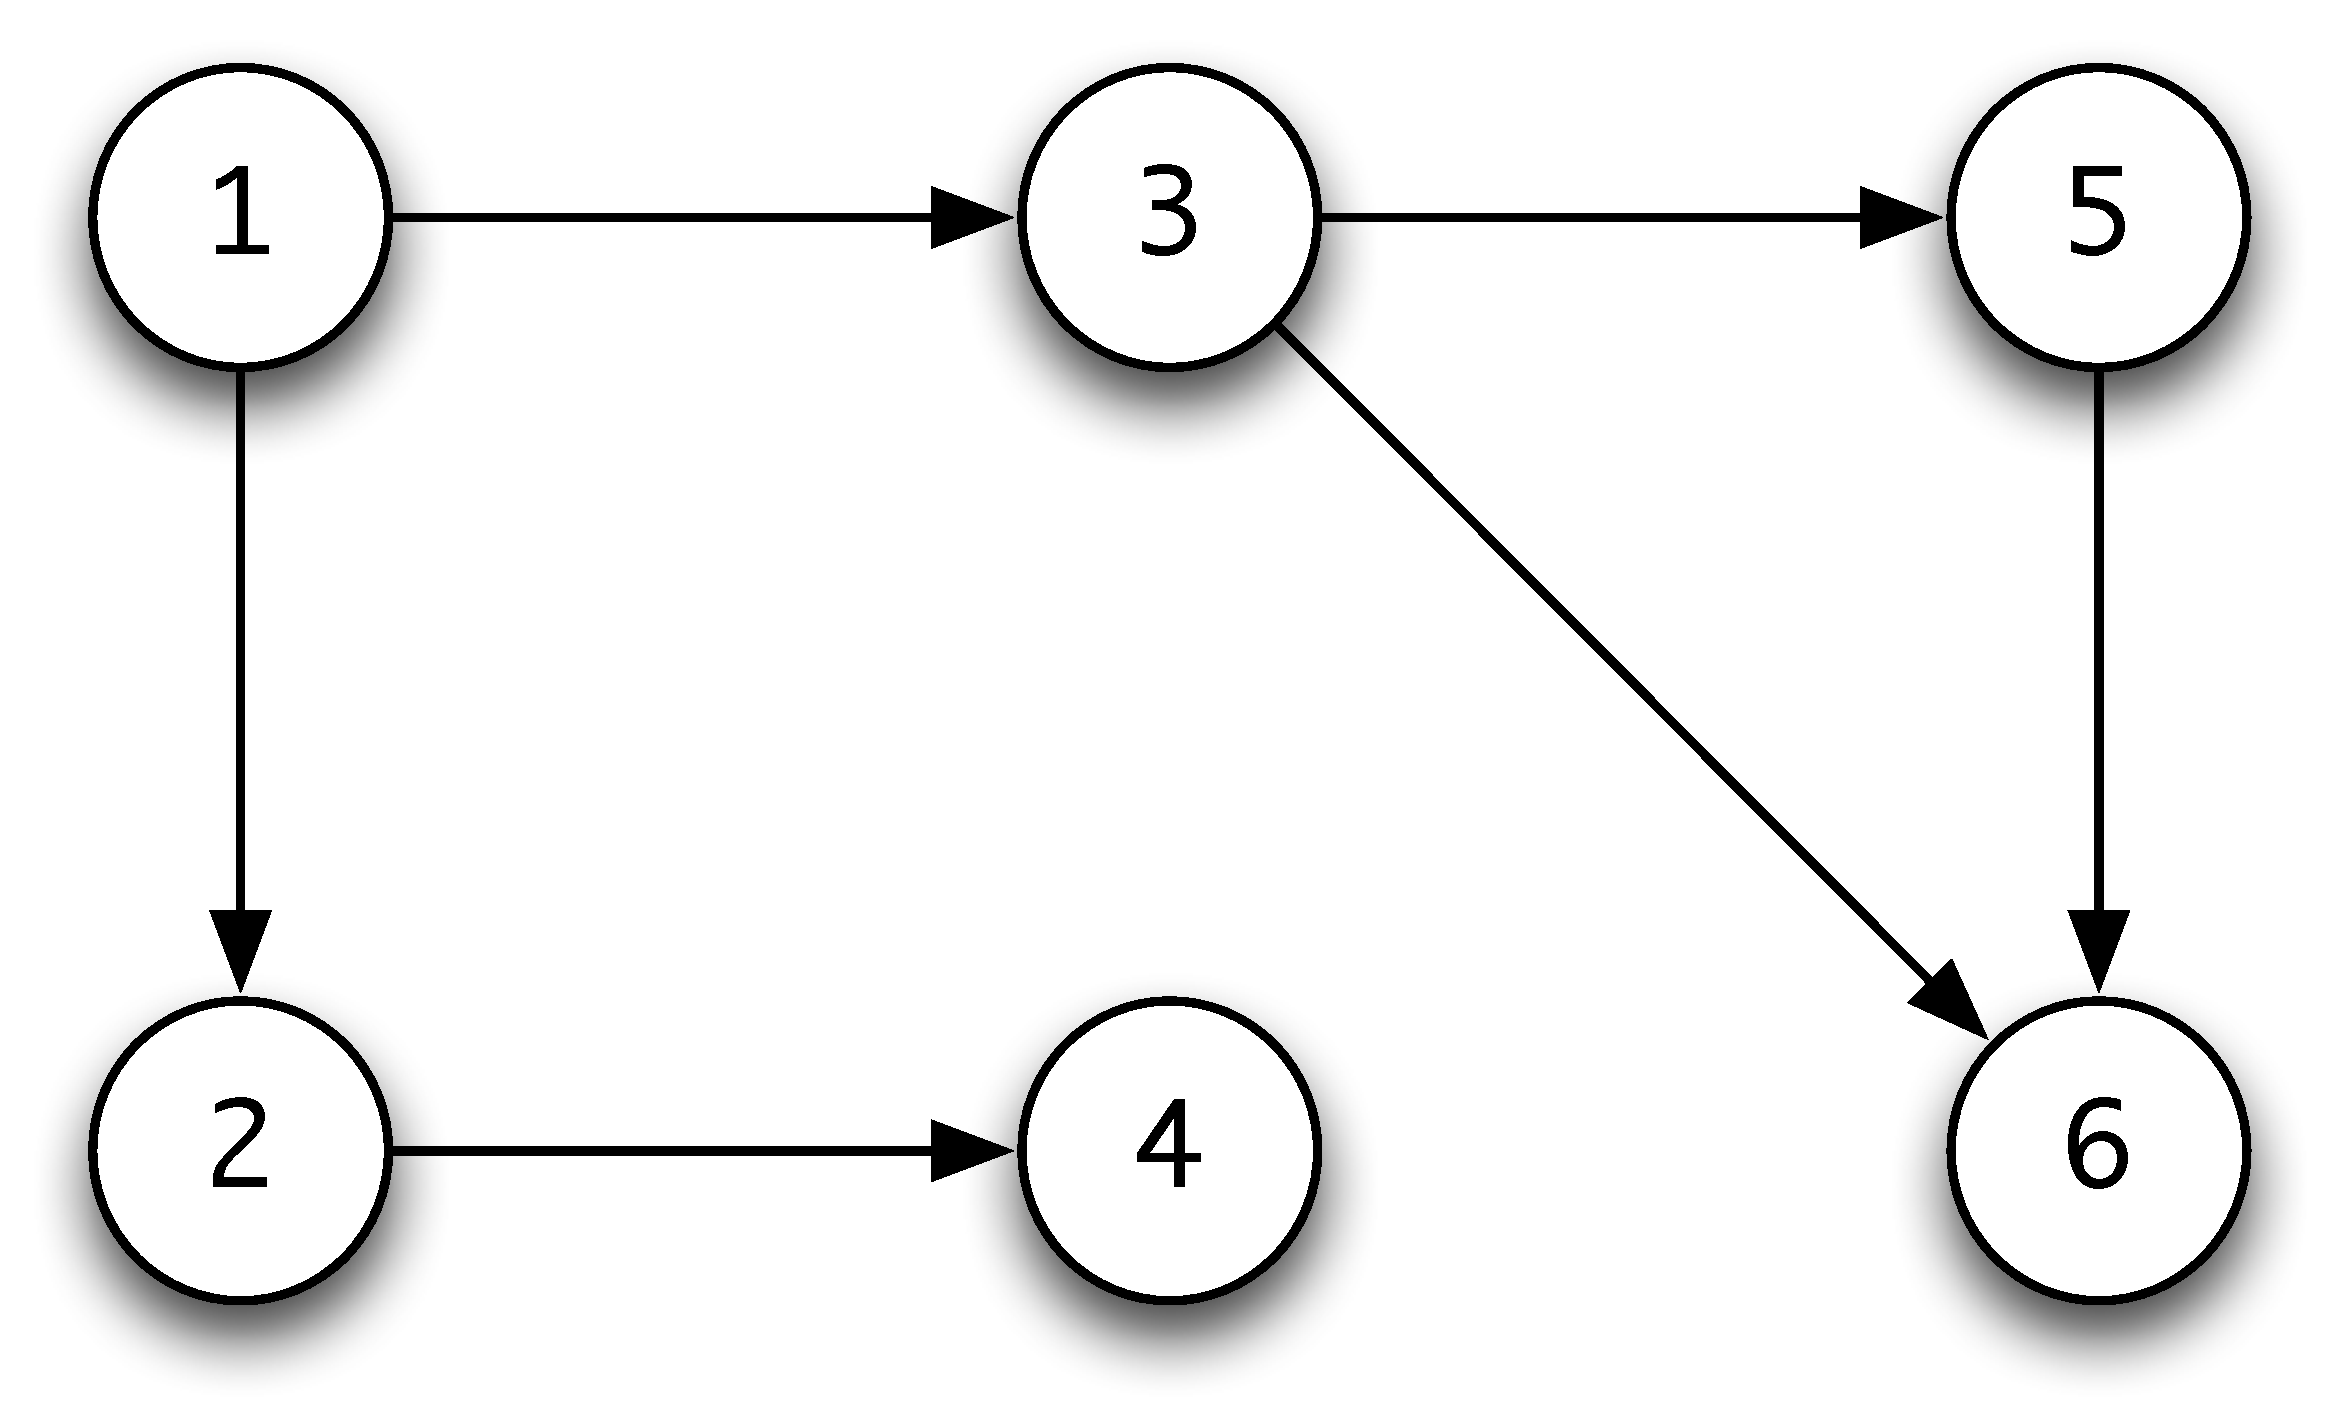
\includegraphics[width=2in]{Pictures/Graph2.pdf}
\end{center} 
\begin{alltt}
graphEx = makeSet [(1,2),(1,3),(2,4),(3,5),(5,6),(3,6)]
\end{alltt}
a route from \texttt{1} to \texttt{4} is the list \texttt{[1,2,4]}. 

We solve a
slightly different problem: find the list of {\em all\/} routes from \texttt{x} to
\texttt{y}; our original problem is solved by taking the head of this list. Note
that as a list is returned, the algorithm allows for the possibility of there
being {\em no\/} route from \texttt{x} to \texttt{y} -- the empty list of routes is
the answer in such a case. This method, which is applicable in many different
situations, is often called the \textbf{list of successes}
\index{list of successes method}
technique: instead of
returning one result, or an error if there is none, we return a list; the
error case is signalled by the empty list. The method also allows for multiple
results to be returned, as we shall see.

How do we solve the new problem? 


\paragraph{Acyclic case.}

For the present
we assume that the graph is \textbf{acyclic}: there is no circular path from
any node back to itself.

\begin{titemize} 
\item The only route from \texttt{x} to \texttt{x} is \texttt{[x]}.
\item A route from \texttt{x} to \texttt{y} will start with a step to one of 
\texttt{x}'s neighbours, \texttt{z} say. The remainder will be a path from
\texttt{z} to \texttt{y}.
\end{titemize}
We therefore look for all paths from \texttt{x} to \texttt{y} going through 
\texttt{z}, for each neighbour \texttt{z} of \texttt{x}.
\begin{alltt}\minx{routes}
routes :: Ord a => Relation a -> a -> a -> [[a]]
routes rel x y
  | x==y        = [[x]]
  | otherwise   = [ x:r | z <- nbhrs rel x ,
                          r <- routes rel z y ]
\end{alltt}
The \texttt{nbhrs} function is defined by
\begin{alltt}\minx{nbhrs}
nbhrs :: Ord a => Relation a -> a -> [a]
nbhrs rel x = flatten (image rel x)
\end{alltt} 
where \texttt{flatten} turns a set into a list.
Now consider the example, where we write \texttt{routes'} for \texttt{routes
graphEx} and \texttt{nbhrs'} for \texttt{nbhrs graphEx},
to make the calculation more readable:
\begin{alltt}
routes' 1 4
\step [ 1:r | z <- nbhrs' 1 , r <- routes' z 4 ]
\step [ 1:r | z <- [2,3] , r <- routes' z 4 ]
\step [ 1:r | r <- routes' 2 4 ] ++ 
    [ 1:r | r <- routes' 3 4 ]\hfill (\dag)
\step [ 1:r | r <- [ 2:s | w <- nbhrs' 2 , s <- routes' w 4 ]]++...
\step [ 1:r | r <- [ 2:s | w <- [4] , s <- routes' w 4 ] ] ++ ...
\step [ 1:r | r <- [ 2:s | s <- routes' 4 4 ] ] ++ ...\hfill (\ddag)
\step [ 1:r | r <- [ 2:s | s <- [[4]] ] ] ++ ...
\step [ 1:r | r <- [ [2,4] ] ] ++ ...
\step [[1,2,4]] ++ ...
\end{alltt}
The head of the list is given by exploring only the first neighbour of 
\texttt{1}, namely \texttt{2}, and its first neighbour, \texttt{4}. In this case 
the search
for a route leads directly to a result. This is not always so. Take the
example of
\begin{alltt}
routes' 1 6 = ...
\step [ 1:r | r <- routes' 2 6 ] ++ 
    [ 1:r | r <- routes' 3 6 ]\hfill (\dag)
\step ...
\step [ 1:r | r <- [ 2:s | s <- routes' 4 6 ] ] ++ 
    [ 1:r | r <- routes' 3 6 ]\hfill (\ddag)
\end{alltt}
Corresponding points in the calculations are marked by \texttt{(\dag)} and
\texttt{(\ddag)}. The search for routes from \texttt{4} to \texttt{6} will {\em fail\/},
though, as \texttt{4} has no neighbours -- we therefore have
\begin{alltt}
\step [] ++ [ 1:r | r <- routes' 3 6 ] = ...
\step [ 1:r | r <- [ 3:s | s <- routes' 5 6 ] ] ++ ...
\step [[1,3,5,6]] ++ ...
\end{alltt}
The effect of this algorithm is to \textbf{backtrack} \index{backtracking}
when a search has
failed: there is no route from \texttt{1} to \texttt{6} via \texttt{2}, so the other
possibility of going through \texttt{3} is explored. This is done  {\em only\/}
when the first possibility is exhausted, however, so lazy evaluation ensures
that this search through `all' the paths turns out to be an efficient method
of finding a single path. Moreover, we don't have to think explicitly about backtracking, it simply falls out from our description of the list of all solutions, evaluated lazily.


\paragraph{General case.}

We assumed at the start of this development that the graph was acyclic, so
that we have no chance of a path looping back on itself, and so of a search
going into a loop. We can make a simple addition to the program to make sure
that only paths without cycles are explored, and so that the program will
work for an arbitrary graph. We add a list argument for the points not to be
visited (again), and so have
\begin{alltt}\minx{routesC}
routesC :: Ord a => Relation a -> a -> a -> [a] -> [[a]]
routesC rel x y avoid
  | x==y        = [[x]]
  | otherwise   = [ x:r | z <- nbhrs rel x \bs{}\bs{} avoid ,
                          r <- routesC rel z y (x:avoid) ]
\end{alltt}
Two changes are made in the recursive case.
\begin{titemize}
\item In looking for neighbours of \texttt{x} we look only for those which are
not in the list \texttt{avoid};
\item in looking for routes from \texttt{z} to \texttt{y}, we exclude visiting both
the elements of \texttt{avoid} and the node \texttt{x} itself. 
\end{titemize}
A search for a route from \texttt{x} to \texttt{y} in \texttt{rel} is given by \texttt{
routesC rel x y []}.
\end{example}

\begin{exerciseone}
\item
Defining \texttt{graphEx2} to be
\begin{alltt} 
makeSet [(1,2),(2,1),(1,3),(2,4),(3,5),(5,6),(3,6)]
\end{alltt}
try calculating
the effect of the original definition on  
\begin{alltt}
routes graphEx 1 4
\end{alltt}
Repeat the calculation with the revised definition which follows:
\begin{alltt}
routes rel x y
  | x==y        = [[x]]   
  | otherwise   = [ x:r | z <- nbhrs rel x ,
                          r <- routes rel z y ,
                          not (elem x r) ]
\end{alltt}
and explain why this definition is not suitable for use on cyclic graphs.
Finally, give a calculation of 
\begin{alltt}
routesC graphEx 1 4 []
\end{alltt}
\index{data-directed programming|)}
\end{exerciseone}


\section{Case study: parsing expressions}
\label{parsing}
\index{case studies!parsing|see{parsing}}
\index{parsing|(}
\index{calculator|(}

We have already seen the definition of \texttt{Expr}, the type of arithmetic
expressions, in Section \ref{recTypes} and in a 
revised version given on page \pageref{modExpr}:
\begin{alltt}
data Expr = Lit Int | Var Var | Op Ops Expr Expr\minx{Expr}
data Ops  = Add | Sub | Mul | Div | Mod\minx{Ops}
\end{alltt}
and showed there how we could calculate
the results of these expressions using the function \texttt{eval}. Chapter
\minx{eval}\minx{Store}
\ref{adt} began with a discussion of how to represent the values held in the
variables using the abstract data type \texttt{Store}. Using these components, we
can build a calculator for simple arithmetical expressions, but the
input is unacceptably crude, as we have to enter members of the \texttt{Expr}
type, so that to add \texttt{2} and \texttt{3}, we are forced to type
%\begin{alltt}
\texttt{Op Add (Lit 2) (Lit 3)}. %\hfill(exp)
%\end{alltt}
What we need to make the input reasonable is a function which performs the
reverse of \texttt{show}: it will take the string \texttt{"(2+3)"} and return the
expression \texttt{Op Add (Lit 2) (Lit 3)}, which is of type \texttt{Expr}. A function like this is called a \textbf{parser} and the process of turning a `flat' string into a structure like an \texttt{Expr} is called \textbf{parsing}.

Constructing a parser for a type like \texttt{Expr} gives a \texttt{read} function
which essentially gives the functionality of the \texttt{Read} class, introduced in
Section \ref{haskellClasses} above. Note, however, that the
\texttt{derived} definition of \texttt{read} for \texttt{Expr} will
parse strings of the form \texttt{"Op Add (Lit 2) (Lit 3)"}, which doesn't help us to build the parser for strings like \texttt{"(2+3)"}.
\index{parsing!and \texttt{read}}

\subsection*{The type of parsers: \texttt{Parse}}
\minx{Parse}

In building a library of parsing functions, we first have to establish the
type we shall use to represent parsers.  Our approach here is again \emph{data directed}: we will look at how a parser is represented as a function of a particular type, and in looking at how particular parsers are constructed we'll again concentrate on how data is transformed through the parsing process.
 
The problem of parsing is to take a list of objects -- of type
\texttt{a} and
characters in our example \texttt{"(2+3)"} -- and from it to extract an object
of some other type, \texttt{b}, in this case \texttt{Expr}. As a first attempt, we
might define the type of parsers thus:
\begin{alltt}
type Parse1 a b = [a] -> b
\end{alltt}
Suppose that \texttt{bracket} and \texttt{number} are the parsers of this type
which recognize brackets and numbers then we have
\begin{alltt}
bracket "(xyz" \step '('
number  "234"  \step 2 {\rm{}or} 23 {\rm{}or} 234{\rm{}?}
bracket "234"  \step {\rm{}no result?}
\end{alltt}
The problem evident here is that a parser can return more than one result --
as in \texttt{number "234"} -- or none at all, as seen in the final case.
Instead of the original type, we suggest
\begin{alltt}
type Parse2 a b = [a] -> [b]
\end{alltt}
where a list of results is returned. In our examples,
\begin{alltt}
bracket "(xyz" \step ['(']
number  "234"  \step [2 , 23 , 234]
bracket "234"  \step []
\end{alltt}
In this case an empty list signals failure to find what was sought, while
multiple results show that more than one successful parse was possible. We
are using the `list of successes' technique again, in fact.

Another problem presents itself. What if we look for a bracket {\em followed
by\/} a number, which we have to do in parsing our expressions? We need to
know the part of the input which remains after the successful parse. Hence we
define
\begin{alltt}\minx{Parse}
type Parse a b = [a] -> [(b,[a])]
\end{alltt}
and our example functions will give
\begin{alltt}
bracket "(xyz" \step [('(' , "xyz")]
number  "234"  \step [(2,"34") , (23,"4") , (234,"")]
bracket "234"  \step []
\end{alltt}
Each element in the output list represents a successful parse. In
\texttt{number "234"} we see three successful parses, each recognizing a number.
In the first, the number \texttt{2} is recognized, leaving \texttt{"34"}
unexamined, for instance.

The type \texttt{ReadS b},\minx{ReadS} which appears in the standard prelude and is used in
defining the \texttt{Read} class, is a special case of the type \texttt{Parse a b} in which
\texttt{[a]} is replaced by \texttt{String}, that is, \texttt{a} is replaced by \texttt{Char}.

\subsection*{Some basic parsers}
\index{parsing!basic parsers}

Now we have established the type we shall use, we can begin to write some
parsers. These and the parser-combining functions are illustrated in Figure
\ref{majParsing}; we go through the definitions now.

The first is a parser which always fails, so accepts nothing. There
are no entries in its output list.
\begin{alltt}\minx{none}
none :: Parse a b
none inp = []
\end{alltt}
On the other hand, we can succeed immediately, without reading any input.
The value recognized is a parameter of the function.
\begin{alltt}
succeed :: b -> Parse a b\minx{succeed} 
succeed val inp = [(val,inp)]
\end{alltt}
More useful is a parser to recognize a single object or token, \texttt{t}, say. We
define
\begin{alltt}
token :: Eq a => a -> Parse a a\minx{token}
token t (x:xs) 
  | t==x        = [(t,xs)]
  | otherwise   = []
token t []      = []
\end{alltt}
More generally, we can recognize (or \texttt{spot}) objects with a particular
property, as represented by a Boolean-valued function.
\begin{alltt}
spot :: (a -> Bool) -> Parse a a\minx{spot}
spot p (x:xs) 
  | p x         = [(x,xs)]
  | otherwise   = []
spot p []       = []
\end{alltt}
These parsers allow us to recognize single characters like a left bracket,
or a single digit,
\begin{alltt}
bracket = token '('
dig     = spot isDigit
\end{alltt}
and indeed, we can define \texttt{token} from \texttt{spot}:
\begin{alltt}
token t = spot (==t)
\end{alltt}
If we are to build parsers for
complex structures like expressions we will
need to be able to combine these simple parsers into more complicated
ones to, for instance, recognize numbers consisting of lists of digits.

\begin{figure}
\begin{alltt}
infixr 5 >*>

type Parse a b = [a] -> [(b,[a])]\minx{Parse}
 
none :: Parse a b\minx{none}
none inp = []
 
succeed :: b -> Parse a b \minx{succeed}
succeed val inp = [(val,inp)]
 
token :: Eq a => a -> Parse a a\minx{token}
token t = spot (==t)
 
spot :: (a -> Bool) -> Parse a a\minx{spot}
spot p (x:xs) 
  | p x         = [(x,xs)]
  | otherwise   = []
spot p []       = []
 
alt :: Parse a b -> Parse a b -> Parse a b\minx{alt}
alt p1 p2 inp = p1 inp ++ p2 inp

(>*>) :: Parse a b -> Parse a c -> Parse a (b,c)\index{\symbol{62}\symbol{42}\symbol{62}@\texttt{\symbol{62}\symbol{42}\symbol{62}}}	
(>*>) p1 p2 inp 
  = [((y,z),rem2) | (y,rem1) <- p1 inp , (z,rem2) <- p2 rem1 ]
 
build :: Parse a b -> (b -> c) -> Parse a c\minx{build}
build p f inp = [ (f x,rem) | (x,rem) <- p inp ]
	
list :: Parse a b -> Parse a [b]\minx{list}
list p = (succeed []) `alt`
         ((p >*> list p) `build` (uncurry (:)))
\end{alltt}
\caption{The major parsing functions.}
\label{majParsing}
\end{figure}

\subsection*{Combining parsers}
\index{parsing!combinators}

Here we build a library of higher-order polymorphic functions, which we then
use to give our parser for expressions. First we have to think about the ways
in which  parsers need to be combined. 

Looking at the expression example, an
expression is {\em either\/} a literal, {\em or\/} a variable {\em or\/} an
operator expression. From parsers for the three sorts of expression, we want
to build a single parser for expressions. For this we use \texttt{alt}
\begin{alltt}
alt :: Parse a b -> Parse a b -> Parse a b\minx{alt}

alt p1 p2 inp = p1 inp ++ p2 inp
\end{alltt}
The parser combines the results of the parses given by parsers \texttt{p1} and
\texttt{p2} into a single list, so a success in either is a success of the
combination. For example,
\begin{alltt}
(bracket `alt` dig) "234" 
\step [] ++ [('2',"34")]
\end{alltt}
the parse by \texttt{bracket} fails, but that by \texttt{dig} succeeds, so the
combined parser succeeds.

For our second function, we look again at the expression example. In
recognizing an operator expression we see a bracket {\em then\/} a number. How
do we put parsers together so that the second is applied to the input that
remains after the first has been applied?

We make this function an operator, as we find that it is often used to combine
a sequence of parsers, and an infix form with defined associativity is most
convenient for this.
\begin{alltt}
infixr 5 >*>

(>*>) :: Parse a b -> Parse a c -> Parse a (b,c)\index{\symbol{62}\symbol{42}\symbol{62}@\texttt{\symbol{62}\symbol{42}\symbol{62}}}

(>*>) p1 p2 inp 
  = [((y,z),rem2) | (y,rem1) <- p1 inp , (z,rem2) <- p2 rem1 ]
\end{alltt}
The values \texttt{(y,rem1)} run through the 
possible results of parsing \texttt{inp} using 
\texttt{p1}. For each of these, we apply \texttt{p2} to 
\texttt{rem1}, which is the input which is unconsumed by \texttt{p1} in that
particular case. The results of the two successful parses, \texttt{y} and 
\texttt{z}, are returned as a pair.

As an example, assume that \texttt{digList} recognizes non-empty
sequences of digits, and
look at \texttt{(digList >*> bracket) "24("}.
Applying \texttt{digList} to the string \texttt{"24("} gives two results,
\begin{alltt}
digList "24(" \step [("2","4(") , ("24","(")]
\end{alltt}
and so \texttt{(y,rem1)} runs through two cases
\begin{alltt}
(digList >*> bracket) "24("
\step [((y,z),rem2) | (y,rem1) <- [("2","4(") , ("24","(")] ,
                    (z,rem2)  <- bracket rem1 ]
\step [(("2",z),rem2)  | (z,rem2)  <- bracket "4(" ] ++
    [(("24",z),rem2) | (z,rem2)  <- bracket "(" ] 
\end{alltt}
Now, \texttt{bracket "4(" \step []}, so fails, giving
\begin{alltt}
\step [] ++ [(("24",z),rem2) | (z,rem2)  <- bracket "(" ] 
\end{alltt}
and
\begin{alltt}
bracket "(" \step [('(',"")]
\end{alltt}
which signals success, and finally gives\begin{alltt}   
\step [(("24",z),rem2) | (z,rem2)  <- [('(',"")] ] 
\step [ (("24",'(') , "") ]
\end{alltt}
This shows we have one successful parse, in which we have recognized the digit list
\texttt{"24"} followed by the left bracket \texttt{'('}.

Our final operation is to change the item returned by a parser, or to 
\texttt{build} something from it. Consider again the case of the parser, \texttt{digList}, which
returns a list of digits. Can we make it return the number which the list of
digits represents? We apply conversion to the results,
thus
\begin{alltt}
build :: Parse a b -> (b -> c) -> Parse a c\minx{build}

build p f inp = [ (f x,rem) | (x,rem) <- p inp ]
\end{alltt}
so in an example, we have
\begin{alltt}
(digList `build` digsToNum) "21a3"
\step [ (digsToNum x,rem) | (x,rem) <- digList "21a3" ]
\step [ (digsToNum x,rem) | (x,rem) <- [("2","1a3"),("21","a3")]]
\step [ (digsToNum "2" , "1a3") , (digsToNum "21" , "a3") ]
\step [ (2,"1a3") , (21,"a3")]
\end{alltt}
Using the three operations or \textbf{combinators} \texttt{alt}, \texttt{>*>} and
\texttt{build} together with the primitives of the last section we will be able to
define all the parsers we require.

As an example, we show how to define a parser
for a \textbf{list} of objects, when we are given
a parser to recognize a single object. There are two sorts of list:
\begin{titemize}
\item A list can be empty, which will be recognized by the parser 
\texttt{succeed []}.
\item Any other list is non-empty, and consists of an object followed by a
list of objects. A pair like this is recognized by \texttt{p >*> list p}; we
then have to turn this pair \texttt{(x,xs)} into the list \texttt{(x:xs)}, for which
we use \texttt{build}, applied to the uncurried form of \texttt{(:)},
which takes its arguments as a pair, and thus converts \texttt{(x,xs)}
to \texttt{(x:xs)}.
\end{titemize}
\begin{alltt}
list :: Parse a b -> Parse a [b]

list p = (succeed []) `alt`
         ((p >*> list p) `build` (uncurry (:)))
\end{alltt}

\begin{exercises}

\item
Define the functions
\begin{alltt}
neList   :: Parse a b -> Parse a [b]
optional :: Parse a b -> Parse a [b]
\end{alltt}
so that \texttt{neList p} recognizes a non-empty list of the objects
which are
recognized by \texttt{p}, and \texttt{optional p} recognizes such an object
{\em optionally\/} -- it may recognize an object or succeed immediately.

\item
Define the function
\begin{alltt}
nTimes :: Integer -> Parse a b -> Parse a [b]
\end{alltt}
so that \texttt{nTimes n p} recognizes \texttt{n} of the
objects recognized by \texttt{p}.
\end{exercises}

\subsection*{A parser for expressions}
\minx{Expr}
\index{parsing!expressions|(}

Now we can describe our expressions and define the parser for them.
Expressions have three forms:
\begin{titemize}%\index{expression type}
\item Literals: \texttt{67}, \texttt{\twid89}, where `\texttt{\twid}' is used for
unary minus.
\item Variables:        \texttt{'a'} to \texttt{'z'}.
\item Applications of the binary operations \texttt{+,*,-,/,\%}, where \texttt{\%}
is used for \texttt{mod}, and \texttt{/} gives integer division. Expressions are
fully bracketed, if compound, thus: \texttt{(23+(34-45))}, and white
space not permitted.
\end{titemize}
The parser has three parts
\begin{alltt}
parser :: Parse Char Expr\minx{parser}
parser = litParse `alt` varParse `alt` opExpParse
\end{alltt}
corresponding to the three sorts of expression. The simplest to define is
\begin{alltt}\minx{varParse}
varParse :: Parse Char Expr
varParse = spot isVar `build` Var

isVar :: Char -> Bool
isVar x = ('a' <= x \&\& x <= 'z')
\end{alltt}
(Here the constructor \texttt{Var} is used as a function taking a character to
the type \texttt{Expr}.)

An operator expression will consist of two expressions joined by an operator,
the whole construct between a matching pair of parentheses:
\label{opExpParse}\begin{alltt}\minx{opExpParse}
opExpParse 
  = (token '(' >*>
     parser    >*>
     spot isOp >*>
     parser    >*>
     token ')') 
     `build` makeExpr
\end{alltt}
where the conversion function takes a nested sequence of pairs, like

\begin{alltt}
('(',(Lit 23,('+',(Var 'x',')'))))
\end{alltt}
into the expression \texttt{Op Add (Lit 23) (Var 'x')}, thus
\begin{alltt}
makeExpr (_,(e1,(bop,(e2,_)))) = Op (charToOp bop) e1 e2
\end{alltt}
Defining the functions \texttt{isOp} and \texttt{charToOp} is left as an
exercise. 

Finally, we look at the case of literals. A number consists of a non-empty
list of digits, with an optional `\texttt{\twid}' at the front. We therefore use
the functions from the exercises of the previous section to say
\begin{alltt}
litParse \minx{litParse}
  = ((optional (token '\twid')) >*>
     (neList (spot isDigit)) 
    `build` (charlistToExpr . uncurry (++)) 
\end{alltt}
Left undefined here is the function \texttt{charlistToExpr} which should convert
a list of characters to a literal integer; this is an exercise for the reader.

\begin{exercises}

\item
Define the functions 
\begin{alltt}
isOp     :: Char -> Bool
charToOp :: Char -> Ops
\end{alltt}
used in the parsing of expressions.


\item
A \textbf{recogniser}\index{recogniser} is like a parser, but simpler: all it needs to do is to recognise whether (the first part of) a string is what we are looking for. Taking a particular example, a recogniser for numbers, \texttt{numberRec}, should behave like this
\begin{alltt}
numberRec "234"  \step{}["34" , "4" , ""]
numberRec "(34"  \step{}[]
\end{alltt}
where the corresponding \texttt{number} parser gives:
\begin{alltt}
number "234"  \step{}[(2,"34") , (23,"4") , (234,"")]
number "(34"  \step{}[]
\end{alltt}
Explain how you could define \texttt{numberRec} from \texttt{number}, and then give a general set of library functions for building recognisers in a similar way to the library for building parsers.



\item
Define the function
\begin{alltt}
charlistToExpr :: [Char] -> Expr
\end{alltt}
so that
\begin{alltt}
charlistToExpr "234" \step{}Lit 234
charlistToExpr "\twid98" \step{}Lit (-98)
\end{alltt}
which is used in parsing literal expressions.

\item
A command to the calculator to assign the value of \texttt{expr} to the variable
\texttt{var} is represented thus
\begin{alltt}
var:expr
\end{alltt}
Give a parser for these commands.

\item
How would you change the parser for numbers if decimal fractions are to be
allowed in addition to integers?

\item
How would you change the parser for variables if names longer than a single
character are to be allowed? 

\item
Explain how you would modify your parser so that the {\em whitespace\/}
characters space and tab can be used in expressions, but would be ignored on
parsing. (Hint: there is a simple pre-processor which does the trick!)

\item 
(Note: this exercise is for those familiar with Backus-Naur
notation for grammars.) 

Expressions without bracketing and allowing the
multiplicative expressions higher binding power are described by the grammar
\begin{alltt}
Expr  ::= Integer | Var | (Expr Ops Expr) |
          Lexpr Mop Mexpr | Mexpr Aop Expr
Lexpr ::= Integer | Var | (Expr Ops Expr)
Mexpr ::= Integer | Var | (Expr Ops Expr) | Lexpr Mop Mexpr
Mop   ::= '*' | '/' | '\%'
Aop   ::= '+' | '-'     
Ops   ::= Mop | Aop
\end{alltt}
Give a Haskell parser for this grammar. Discuss the associativity of the
operator `\texttt{-}' in this grammar.
\end{exercises}
\subsection*{The top-level parser}
\index{parsing!top-level parser}

The parser defined in the last section, \texttt{parser} is of type 
\begin{alltt}
[Char] -> [ (Expr,[Char]) ]
\end{alltt}
yet what we need is to convert this to a function taking a string to the
expression it represents. We therefore define the function
\begin{alltt}
topLevel :: Parse a b -> b -> [a] -> b\minx{topLevel}
topLevel p defaultVal inp
  = case results of
      [] -> defaultVal
      _  -> head results
    where
    results = [ found | (found,[]) <- p inp ]
\end{alltt}
The parse \texttt{p inp} is successful if the result contains at least one parse
(the second case) in which all the input has
been read (the test given by the pattern match to \texttt{(found,[])}). If this
happens, the first value \texttt{found} is returned; otherwise (the first case) we return the default value of type \texttt{b}, \texttt{defaultVal}, which in our case study will be the default command, \texttt{Null}.

We can define the type of commands thus
\begin{alltt}\minx{Command}
data Command = Eval Expr | Assign Var Expr | Null
\end{alltt}
which are intended to cause 
\begin{titemize}
\item the evaluation of the expression,
\item the assignment of the value of the expression to the variable, and
\item no effect.
\end{titemize}
If the assignment command takes the form \texttt{var:expr}, then it is not
difficult to design a parser for this type,
\begin{alltt}\minx{commandParse}
commandParse :: Parse Char Command
\end{alltt}
We will assume this has been built when we revisit the calculator example
below.
\index{calculator|)}

\beware{Testing parsers in QuickCheck}{
If we're able to generate random terms of type \texttt{Expr} or \texttt{Command} then we can write some elegant QuickCheck tests by `round tripping' from expression to string -- via a \texttt{show} function -- and then back to an expression by parsing the string. We show how to generate these random terms in Section \ref{qcGens}.
}

\subsection*{Conclusions}

The type of parsers \texttt{Parse a b} with the functions
\begin{alltt}\index{parsing!library}\minx{Parse}
none     :: Parse a b
succeed  :: b -> Parse a b 
spot     :: (a -> Bool) -> Parse a a
alt      :: Parse a b -> Parse a b -> Parse a b
>*>      :: Parse a b -> Parse a c -> Parse a (b,c)
build    :: Parse a b -> (b -> c) -> Parse a c
topLevel :: Parse a b -> [a] -> b
\end{alltt}
allow us to construct so-called recursive descent parsers in a
straightforward way. It is worth looking at the aspects of the language we
have exploited.
\begin{titemize}
\item The type \texttt{Parse a b} is represented by a function type, so that
all the parser combinators are higher order functions.
\item Because of polymorphism, we do not need to be specific about
either the input or the output type of the parsers we build. 
\itempar
In our example
we have confined ourselves to inputs which are strings of characters, but
they could have been {\em tokens\/} of any other type, if required: we might
take the tokens to be {\em words\/} which are then parsed into sentences, for
instance. 
\itempar
More importantly in our example, we can return objects of any
type using the same combinators, and in the example we returned lists and
pairs as well as simple characters and expressions.
\item Lazy evaluation plays a role here also. The possible parses we build
are generated {\em on demand\/} as the alternatives are tested. The parsers
will backtrack\index{backtracking} through the different options until a successful one is found.
\end{titemize}
Building general libraries like this parser library is one of the major
advantages of using a modern functional programming language 
with the facilities mentioned
above. From a\index{advantages of functional programming}
toolkit like this it is possible to build a whole range of parsers and
language processors which can form the front ends of systems of all sorts.

We will return to a discussion of parsing in Chapter 18; note
also that we could make the type of \texttt{Parse a b} into an abstract
data type, along the lines discussed in Chapter \ref{adt}. On the other
hand, it would also be useful to leave the implementation open to
extension by users, which is the way in which other Haskell libraries
are made available.

\begin{exercises}

\item
Define a parser which recognizes strings representing Haskell lists of integers,
like
\texttt{"[2,-3,45]"}.

\item
Define a parser to recognize simple sentences of English, with a subject,
verb and object. You will need to provide some vocabulary, \texttt{"cat"},
\texttt{"dog"}, and so on, and a parser to recognize a string. You will also need
to define a function
\begin{alltt}
tokenList :: Eq a => [a] -> Parse a [a]
\end{alltt}
so that, for instance,
\begin{alltt}
tokenList "Hello" "Hello Sailor" \step [ ("Hello"," Sailor") ]
\end{alltt}


\item
Define the function
\begin{alltt}
spotWhile :: (a -> Bool) -> Parse a [a]
\end{alltt}
whose parameter is a function which tests elements of the input type, and
returns the longest initial part of the input, all of whose elements have the
required property. For instance
\begin{alltt}
spotWhile digit "234abc"  \step [ ("234","abc") ]
spotWhile digit "abc234"  \step [ ([],"abc234") ]
\end{alltt}
\index{parsing|)}
\index{parsing!expressions|)}

\end{exercises}
\section[Infinite lists]{Infinite lists}
\label{infLists}
\index{lists!infinite|(}
\markright{Infinite lists}

One important consequence of lazy evaluation is that it is
possible for the language to describe \textbf{infinite} structures. These
would require an infinite amount of time to evaluate fully, but under lazy
evaluation it is possible to compute with only portions of a data structure rather than
the whole object.  Any recursive
type will contain infinite objects; we concentrate on lists here, as these are
by far the most widely used infinite structures.

In this section we look at a variety of examples, starting with simple
one-line definitions and moving to an examination
of random numbers to be used in our
simulation case study.
The simplest examples of infinite lists are constant lists like
\begin{alltt}\minx{ones}
ones = 1 : ones
\end{alltt}
Evaluation of this in a Haskell system
produces a list of ones, indefinitely. This
can be \textbf{interrupted}\index{evaluation!interruption} in GHCi
by typing \texttt{Ctrl-C}; this produces the result
\begin{alltt}
[1,1,1,1,1,1,1,\^{}C,1,1,1,Interrupted.
\end{alltt}
We can sensibly evaluate functions applied to \texttt{ones}. If we define
\begin{alltt}
addFirstTwo :: [Integer] -> Integer
addFirstTwo (x:y:zs) = x+y
\end{alltt}
then applied to \texttt{ones} we have
\begin{alltt}
addFirstTwo ones
\step addFirstTwo (1:ones) 
\step addFirstTwo (1:1:ones)
\step 1+1
\step 2
\end{alltt} 
Built into the system are the lists \texttt{[n ..\ ]}, \texttt{[n,m ..\ ]}, so that
\begin{alltt}
[3 ..\ ]   = [3,4,5,6,...
[3,5 ..\ ] = [3,5,7,9,...
\end{alltt}
We can define these ourselves:
\begin{alltt}
from :: Integer -> [Integer]
from n = n : from (n+1)

fromStep :: Integer -> Integer -> [Integer]
fromStep n m = n : fromStep (n+m) m
\end{alltt}
and an example evaluation gives
\begin{alltt}
fromStep 3 2
\step 3 : fromStep 5 2
\step 3 : 5 : fromStep 7 2
\step ...
\end{alltt}
These functions are also defined over any instance of the
\texttt{Enum}\minx{Enum} class;
details can be found in standard prelude.

\index{list comprehensions!infinite}
List comprehensions can also define infinite lists. The list of {\em all\/}
Pythagorean triples\index{Pythagorean triple} -- whole numbers which can the sides of a right-angled triangle -- 
is given by selecting \texttt{z} in \texttt{[2 ..\ ]}, and
then selecting suitable values of \texttt{x} and \texttt{y} below that.
\begin{alltt}\minx{pythagTriples}
pythagTriples =
  [ (x,y,z) | z <- [2 ..\ ] , y <- [2 ..\ z-1] , 
              x <- [2 ..\ y-1] , x*x + y*y == z*z ]
pythagTriples
= [(3,4,5),(6,8,10),(5,12,13),(9,12,15),(8,15,17),(12,16,20),...
\end{alltt}
The powers of an integer are given by
\begin{alltt}
powers :: Integer -> [Integer]
powers n = [ n\^{}x | x <- [0 ..\ ] ] 
\end{alltt}
and this is a special case of the prelude function \texttt{iterate}, which gives the
infinite list
\begin{alltt}
[ x , f x , .. , \superscr{f}{n} x , ..
\end{alltt}  
\begin{alltt}
iterate :: (a -> a) -> a -> [a]\minx{iterate}
iterate f x = x : iterate f (f x)
\end{alltt}

\begin{example}
\subsubexample*{1. Generating prime numbers}
\index{numbers!prime}

A positive integer greater than one is \textbf{prime} if it is divisible only by
itself and one. 
The {\em Sieve of Eratosthenes} -- \index{Eratosthenes}
an algorithm known for over two
thousand years -- works by cancelling out all the multiples of numbers, once
they are established as prime. The primes are the only elements which
remain in the list. The process is illustrated in Figure \ref{sievePic}.
\begin{figure}
\begin{center}
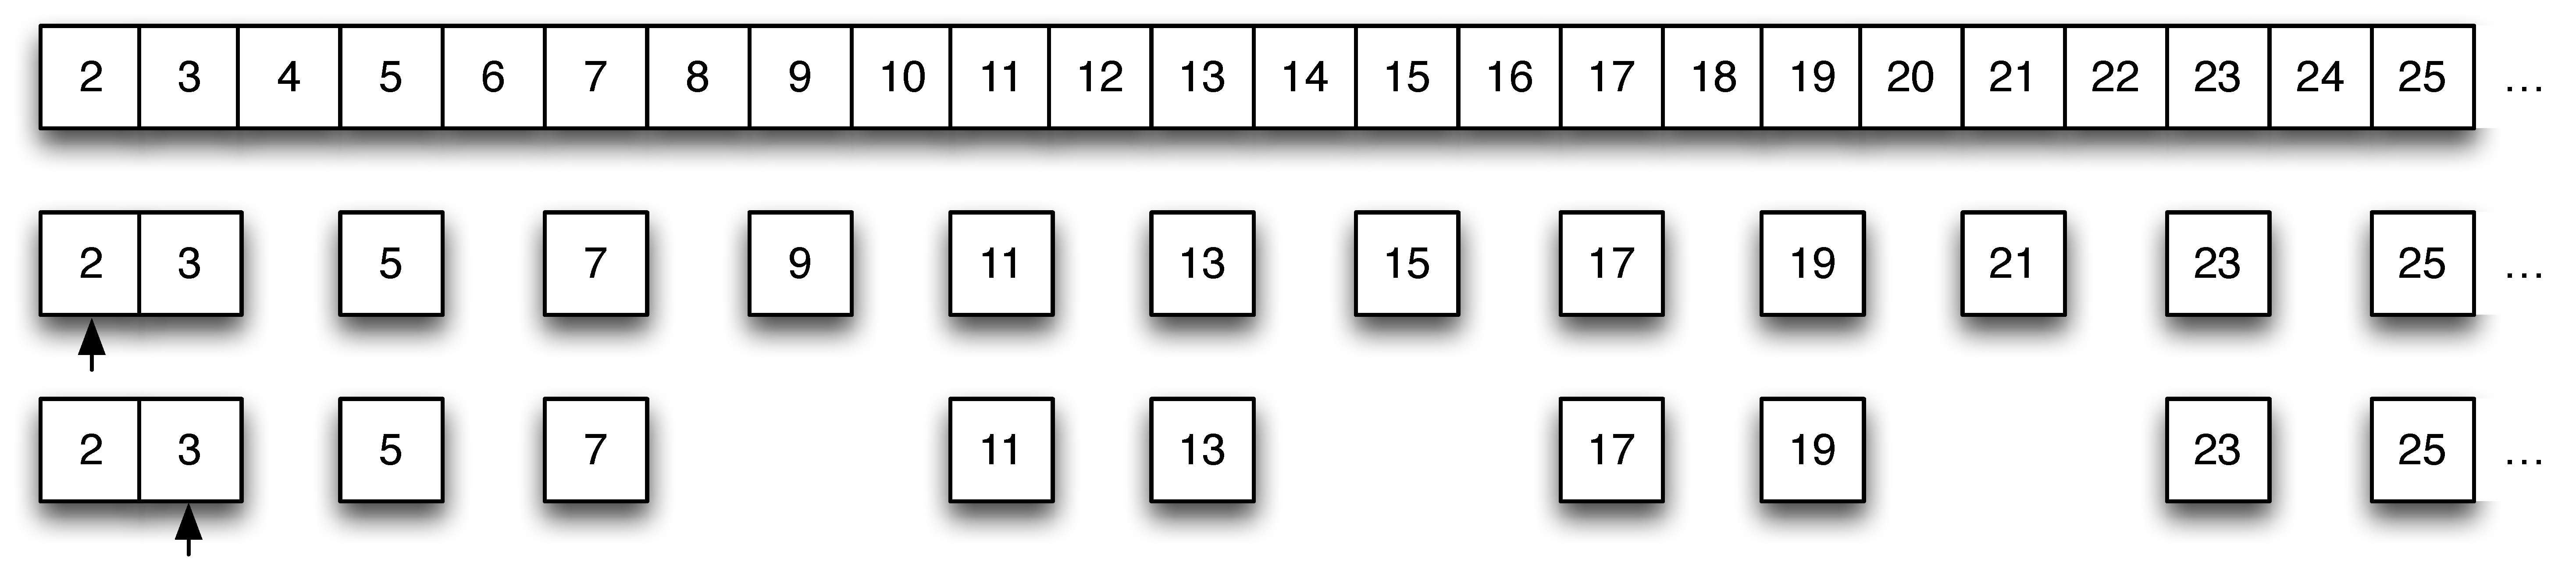
\includegraphics[width=5in]{Pictures/Sieve.pdf}
\end{center} 
\caption{The Sieve of Eratosthenes.}
\label{sievePic}
\end{figure}

We begin with the list of numbers starting at \texttt{2}. The head is
\texttt{2}, and we remove all the multiples of \texttt{2} from the list. The head
of the remainder of the list, \texttt{3}, is prime, since it was not removed in
the sieve by \texttt{2}. We therefore sieve the remainder of the list of
multiples of \texttt{3}, and repeat the process indefinitely. 
As a Haskell definition, we write
\begin{alltt}\minx{primes}\minx{sieve}
primes :: [Integer]

primes       = sieve [2 ..\ ]
sieve (x:xs) = x : sieve [ y | y <- xs , y `mod` x > 0]
\end{alltt}
where we test whether \texttt{x} divides 
\texttt{y} by evaluating \texttt{y `mod` x}; \texttt{y} is a multiple of \texttt{x} if this
value is zero. Beginning the evaluation, we have
\begin{alltt}
primes 
\step sieve [2 ..\ ]
\step 2 : sieve [ y | y <- [3 ..\ ] , y `mod` 2 > 0]
\step 2 : sieve (3 : [ y | y <- [4 ..\ ] , y `mod` 2 > 0])
\mbox{\texttt{\step 2 : 3 : sieve [ z | z <- [ y | y <- [4 ..\ ] , y `mod` 2 > 0],}}
                      z `mod` 3 > 0]  
\step ...
\step 2 : 3 : sieve [ z | z <- [5,7,9...] , z `mod` 3 > 0]  
\step ...
\step 2 : 3 : sieve [5,7,11,...]  
\step ...
\end{alltt}
Can we use \texttt{primes} to test for a number being a prime? If we evaluate 
\texttt{member primes 7} we get the response \texttt{True},
while \texttt{member primes 6} gives no answer. This is because an 
infinite number of elements have to be checked before we conclude that
\texttt{6} is not in the list. The problem is that \texttt{member} cannot use the
fact that \texttt{primes} is ordered. This we do in \texttt{memberOrd}.
\begin{alltt}\minx{memberOrd}
memberOrd :: Ord a => [a] -> a -> Bool
memberOrd (x:xs) n
  | x<n         = memberOrd xs n
  | x==n        = True
  | otherwise   = False
\end{alltt}
The difference here is in the final case: if the head of the list (\texttt{x)}
is greater
than the element we seek (\texttt{n}),
the element cannot be a member of the ordered list.
Evaluating the test again,
\begin{alltt}
memberOrd [2,3,5,7,11,...] 6
\step memberOrd [3,5,7,11,...] 6  
\step memberOrd [5,7,11,...] 6  
\step memberOrd [7,11,...] 6 
\step False
\end{alltt}
\vspace{5pt}

\subsubexample*{2. Generating random numbers}
\index{numbers!random}


Many computer systems require us to generate `random' numbers, one after
another. Our queuing simulation is a particular example upon which we focus
here, after looking at the basics of the problem.

No Haskell program can produce a truly random sequence; after all, we
want to be able to predict the behaviour of our programs, and randomness is
inherently unpredictable. What we can do, however, is generate a {\bf
pseudo-random}\index{pseudo-random numbers} sequence of natural numbers, smaller than \texttt{modulus}. 
This \textbf{linear congruential method} works by starting with a \texttt{seed},
and then by getting the next element of the sequence from the previous value
thus
\begin{alltt}
nextRand :: Integer -> Integer
nextRand n = (multiplier*n + increment) `mod` modulus
\end{alltt}
A (pseudo-)random sequence is given by iterating this function,
\begin{alltt}
randomSequence :: Integer -> [Integer]\minx{randomSequence}
randomSequence = iterate nextRand
\end{alltt}
Given the values
\begin{alltt}
seed       = 17489
multiplier = 25173
increment  = 13849
modulus    = 65536
\end{alltt}
the sequence produced by \texttt{randomSequence seed} begins
\begin{alltt}
[17489,59134,9327,52468,43805,8378,...
\end{alltt}
The numbers in this sequence, which range from \texttt{0} to \texttt{65535}, all
occur with the same frequency. What are we to do if instead we want the
numbers to come in the (integer) range \texttt{a} to \texttt{b} inclusive? We need
to scale the sequence, which is achieved by a \texttt{map}:
\begin{alltt}\minx{scaleSequence}
scaleSequence :: Integer -> Integer -> [Integer] -> [Integer]
scaleSequence s t
  = map scale
    where
    scale n = n `div` denom + s
    range   = t-s+1
    denom   = modulus `div` range
\end{alltt}
The original range of numbers \texttt{0} to \texttt{modulus-1} is split into 
\texttt{range} blocks, each of the same length. The number \texttt{s} is assigned to
values in the first block, \texttt{s+1} to values in the next, and so on.

In our simulation example, we want to generate for each arrival the length of 
service that person will need on being served. For illustration, we suppose
that they range from \texttt{1} to \texttt{6} minutes, but that they are supposed
to happen with different probabilities.
\begin{center}
\begin{tabular}{|l||c|c|c|c|c|c|}
\hline
Waiting time & \mi 1 & \mi 2 & \mi 3 & \mi 4 & \mi 5 & \mi 6 \\ \hline
Probability & \mi 0.2 & \mi 0.25 & \mi 0.25 & \mi 0.15 & \mi 0.1 & \mi 0.05 \\
\hline 
\end{tabular}
\end{center}
We need a function to turn such a distribution into a transformer of
infinite lists. Once we have a function transforming individual values, we
can \texttt{map} it along the list.

We can represent a distribution of objects of type \texttt{a} by a list of type
\texttt{[(a,Float)]}, where we assume that the numeric entries add up to one.  Our
function transforming individual values will be
\begin{alltt}
makeFunction :: [(a,Float)] -> (Float -> a)\minx{makeFunction}
\end{alltt}
so that numbers in the range \texttt{0} to \texttt{65535} are transformed into
items of type \texttt{a}. The idea of the function 
is to give the following ranges to the entries for the list above.
\begin{center}
\begin{tabular}{|l||c|c|c|c|}
\hline
Waiting time & \mi 1 & \mi 2 & \mi 3 & \mi \ldots  \\ \hline
Range start& \mi 0 & \mi (m*0.2)+1 & 
\mi (m*0.45)+1 & \mi \ldots  \\ \hline 
Range end& \mi m*0.2 & \mi m*0.45 & 
\mi m*0.7 & \mi \ldots  \\ \hline 
\end{tabular}
\end{center}
where \texttt{m} is used for \texttt{modulus}.
The definition follows:
\begin{alltt}
makeFunction dist = makeFun dist 0.0

makeFun ((ob,p):dist) nLast rand
  | nNext >= rand \&\& rand > nLast     
        = ob
  | otherwise                           
        = makeFun dist nNext rand
          where
          nNext = p*fromIntegral modulus + nLast
\end{alltt}
The \texttt{makeFun} function has an extra argument, which carries the position
in the range \texttt{0} to \texttt{modulus-1} reached so far in the search; it is
initially zero. The \texttt{fromIntegral} function used here converts an \texttt{Int} to
an equivalent \texttt{Float}.

The transformation of a list of random numbers is given by
\begin{alltt}
map (makeFunction dist)
\end{alltt}
and the random distribution of waiting times we require begins
thus
\begin{alltt}
map (makeFunction dist . fromIntegral) (randomSequence seed)
= [2,5,1,4,3,1,2,5,4,2,2,2,1,3,2,5,...
\end{alltt}
with \texttt{6} first appearing at the \texttt{35}th position.


A full library for generating random numbers and random data for other types is given in  
\texttt{System.Random}.\minx{System.Random}

\begin{figure}[t]
\beware{Infinite list generators}{\index{list comprehensions!infinite generators}%
\index{pitfalls!infinite list generators}%
The list comprehension \texttt{pythagTriples2}, intended to produce the list of
all Pythagorean triples, instead produces {\em no\/} output to the prompt. 
\index{Pythagorean triple}
\begin{alltt}
pythagTriples2 =
\end{alltt}
\vspace*{-17pt}
\begin{alltt}
\ \ =\ [ (x,y,z) | x <- [2 .. ] ,
\end{alltt}
\vspace*{-17pt}
\begin{alltt}
\ \ \ \ \ \ \ \ \ \ \ \ \ \ \ \ y <- [x+1 .. ] ,
\end{alltt}
\vspace*{-17pt}
\begin{alltt}
\ \ \ \ \ \ \ \ \ \ \ \ \ \ \ \ z <- [y+1 .. ] ,
\end{alltt}
\vspace*{-17pt}
\begin{alltt}
\ \ \ \ \ \ \ \ \ \ \ \ \ \ \ \ x*x + y*y == z*z ]
\end{alltt}
The
problem is in the order of choice of the elements. The first choice for 
\texttt{x} is \texttt{2}, and for \texttt{y} is \texttt{3}; given this, 
there are an infinite
number of values to try for \texttt{z}: \texttt{4}, \texttt{5} and so
on, indefinitely. We therefore never try any of the other choices for
\texttt{x} or \texttt{y}, among which the triples lie.

Two options present themselves. First we can redefine the solution, as
in the original
\texttt{pythagTriples}, so that it involves only one infinite list.
Alternatively, we can try to write a function which returns all pairs of 
elements from two infinite lists:
\begin{alltt}
infiniteProduct :: [a] -> [b] -> [(a,b)]
\end{alltt}
This is left as an exercise. Using such a function it is possible to adapt the
definition of \texttt{pythagTriples2} to make it give all the Pythagorean triples.
}
\end{figure}

\end{example}
\begin{exercises}

\item 
Define the infinite lists of factorial and Fibonacci numbers, 
\begin{alltt}
factorial = [1,1,2,6,24,120,720,...]
fibonacci = [0,1,1,2,3,5,8,13,21,...]
\end{alltt}

\item
Give a definition of the function
\begin{alltt}
factors :: Int -> [Int]
\end{alltt}
which returns a list containing the factors of a positive integer. For
instance,
\begin{alltt}
factors 12 = [1,2,3,4,6,12]
\end{alltt}
Using this function or otherwise, define the list of numbers whose only prime
factors are \texttt{2}, \texttt{3} and \texttt{5}, the so-called \textbf{Hamming numbers}:
\index{Hamming numbers}\label{HamNos}
\begin{alltt}
hamming = [1,2,3,4,5,6,8,9,10,12,15,...
\end{alltt}

\item
Define the function
\begin{alltt}
runningSums :: [Int] -> [Int]
\end{alltt}
which calculates the running sums
\begin{alltt}
[0,\subscr{a}{0},\subscr{a}{0}+\subscr{a}{1},\subscr{a}{0}+\subscr{a}{1}+\subscr{a}{2},...
\end{alltt}
of a list
\begin{alltt}
[\subscr{a}{0},\subscr{a}{1},\subscr{a}{2},...
\end{alltt}

\item
Define the function \texttt{infiniteProduct} specified above, and use it to
correct the definition of \texttt{pythagTriples2}.
\end{exercises}
\section{Why infinite lists?}
\label{whyInfLis}
\index{design!and infinite lists|(}
\index{lists!infinite!why?}
\index{infinite lists|see{lists, infinite}}

Haskell supports infinite lists and other infinite structures, 
and we saw in the last section that we could define a number of quite
complicated
lists, like the list of prime numbers, and lists of random numbers. The
question remains, though, of whether these lists are anything other than a
curiosity. There are two arguments which show their importance in functional
programming.

First, an infinite version of a program can be more \textbf{abstract}, and so simpler
\index{abstraction}
to write. Consider the problem of finding the \texttt{n}th prime number, using the
Sieve of Eratosthenes. If we work with finite lists, we need to know in
advance how large a list is needed to accommodate the first \texttt{n} primes; if
we work with an infinite list, this is not necessary: only that part of the
list which is needed will be generated as computation proceeds.\looseness=1

In a similar way, the random numbers given by \texttt{randomSequence seed}
provided an unlimited resource: we can take as many random numbers from the
list as we require. There needs to be no decision at the start of programming
as to the size of sequence needed. (These arguments are rather like those for
\textbf{virtual memory} in a computer. It is often the case that predicting
the memory use of a program is possible, but tiresome; virtual memory makes
this unnecessary, and so frees the programmer to proceed with other tasks.)

The second argument is of wider significance, and can be seen by re-examining
the way in which we generated random numbers. We generated an infinite list
by means of \texttt{iterate}, and we transformed the values using \texttt{map};
these operations are pictured in Figure \ref{processes1}
as a generator of and a transformer of lists of values. These
values are shown in the dashed boxes.\index{lists!as
processes}\index{processes}
These components can then be linked together, giving more complex
combinations, as in Figure \ref{processes2}.
\begin{figure}[t]
\begin{center}
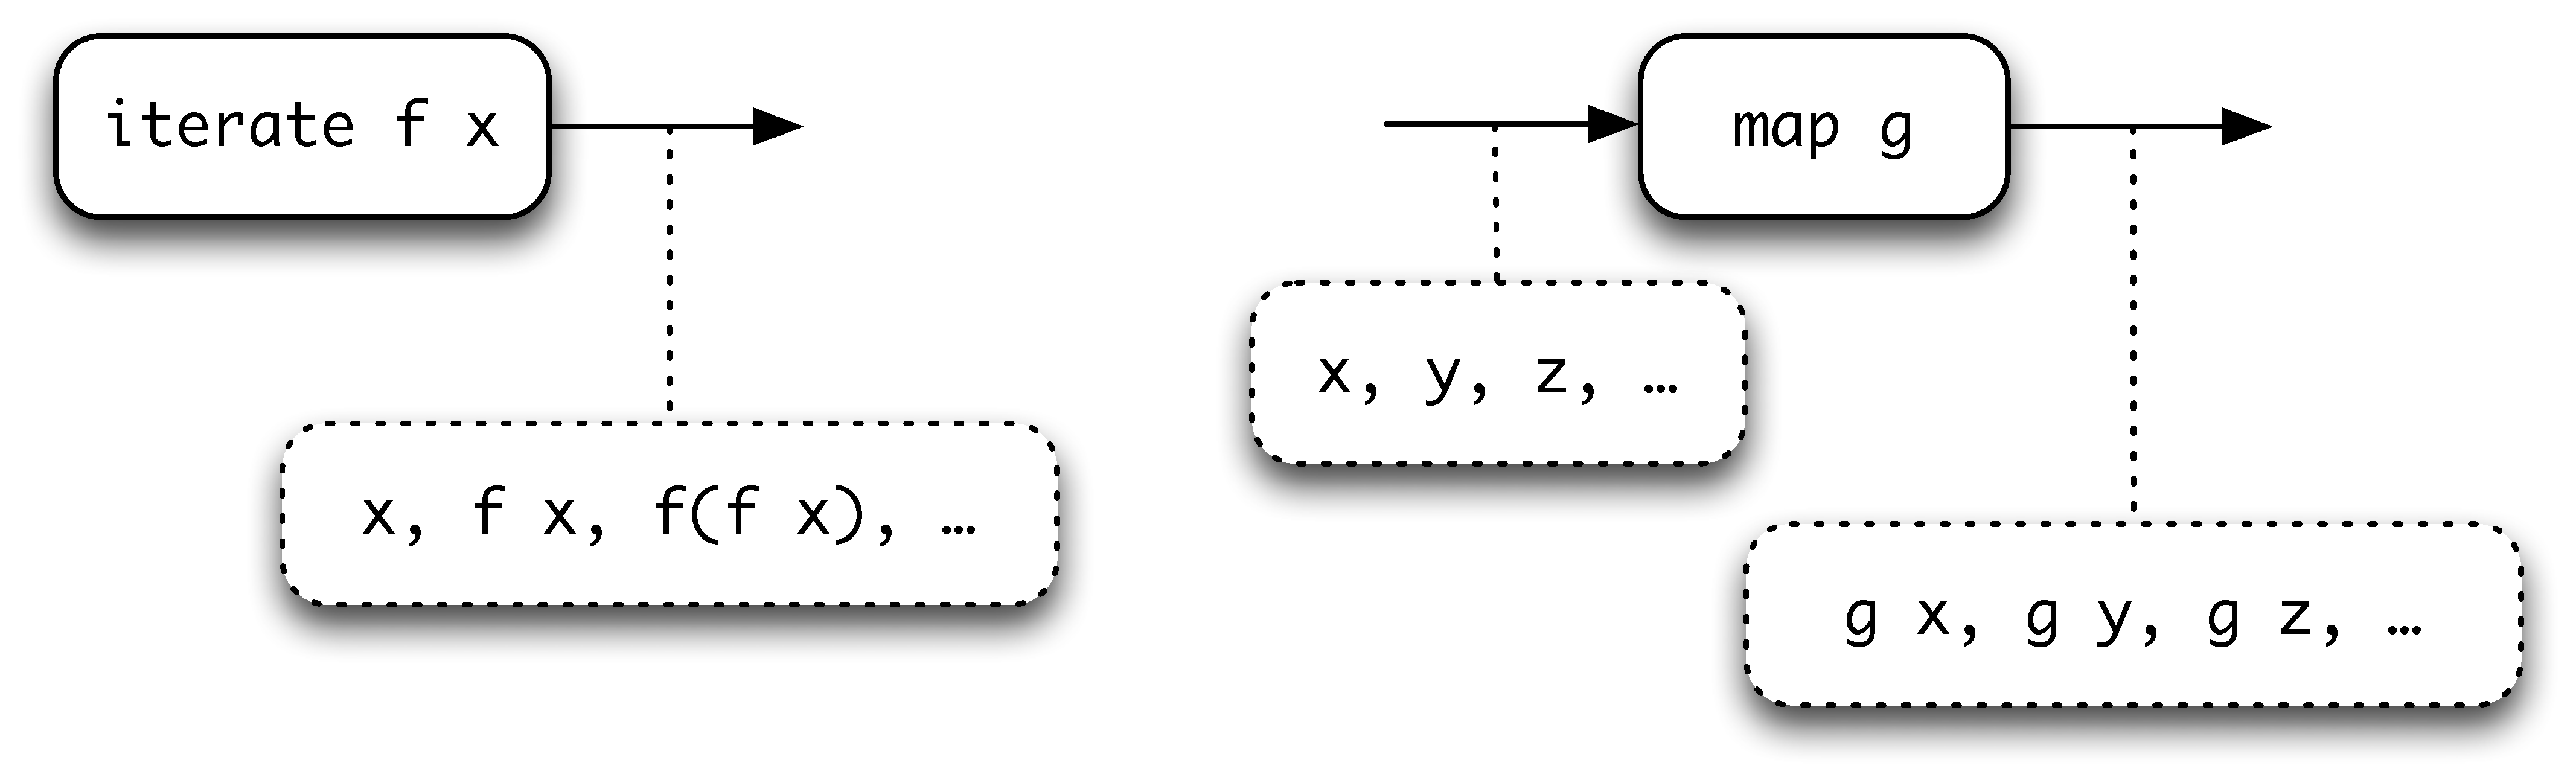
\includegraphics[width=5in]{Pictures/Processes1.pdf}
\end{center} 
\caption{A generator and a transformer.}
\label{processes1}
\end{figure}
\begin{figure}[t]
\begin{center}
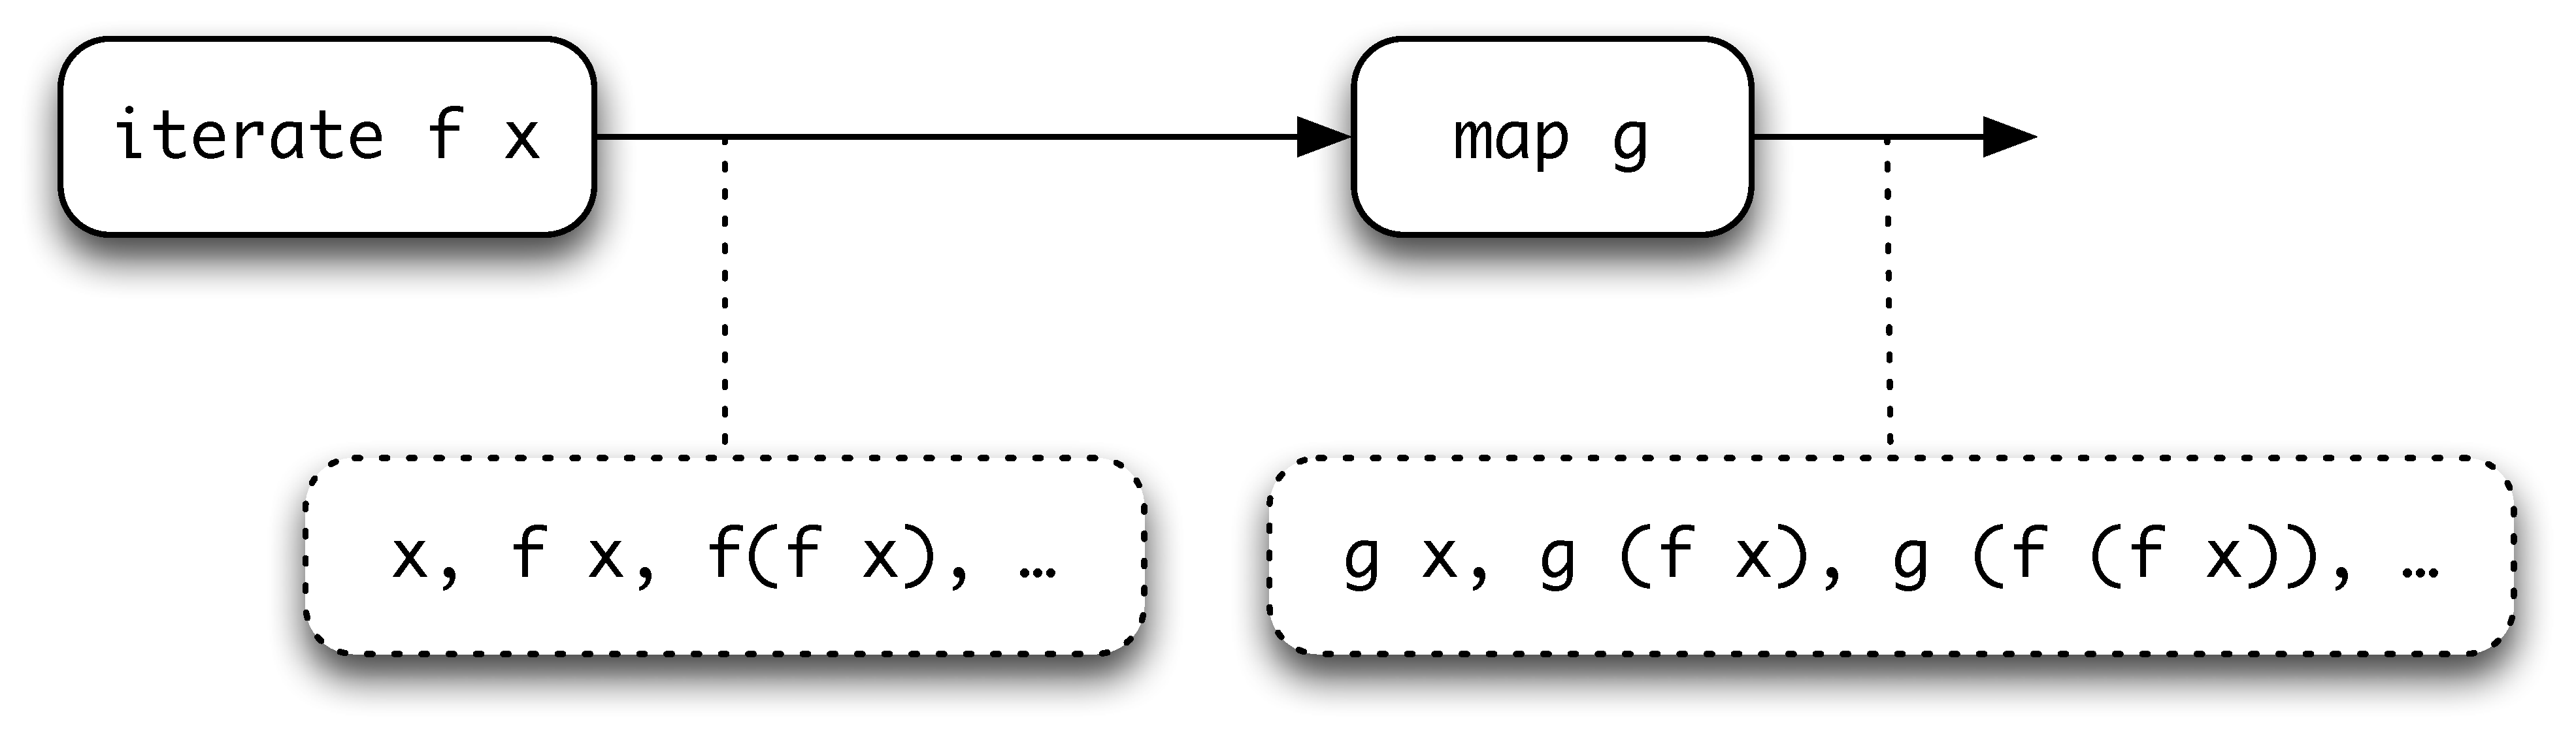
\includegraphics[width=5in]{Pictures/Processes2.pdf}
\end{center} 
\caption{Linking processes together.}
\label{processes2}
\end{figure}
This approach \textbf{modularizes} the generation of values in a distribution in
an interesting way. We have separated the generation of the values from
their transformation, and this means we can change each part independently of
the other.

Once we have seen the view of infinite lists as the links between
processes, other combinations suggest themselves, and in particular we can
begin to write process-style programs which involve \textbf{recursion}.
\index{recursion}

Among the exercises in the last section was the problem of finding the running
sums
\begin{alltt}
[0,\subscr{a}{0},\subscr{a}{0}+\subscr{a}{1},\subscr{a}{0}+\subscr{a}{1}+\subscr{a}{2},...
\end{alltt}
of the list \texttt{[\subscr{a}{0},\subscr{a}{1},\subscr{a}{2},...}. Given the
sum up to \texttt{\subscr{a}{k}}, say, we get the next sum by adding the next
value in the input, \texttt{\subscr{a}{k+1}}. It is as if we {\em feed the sum
back\/}\index{feedback}
into the process to have the value \texttt{\subscr{a}{k+1}} added. This
is precisely the effect of the network of processes in Figure \ref{sumStream}, where
the values passing along the links are shown in the dotted boxes.\looseness=1
\begin{figure}
\begin{center}
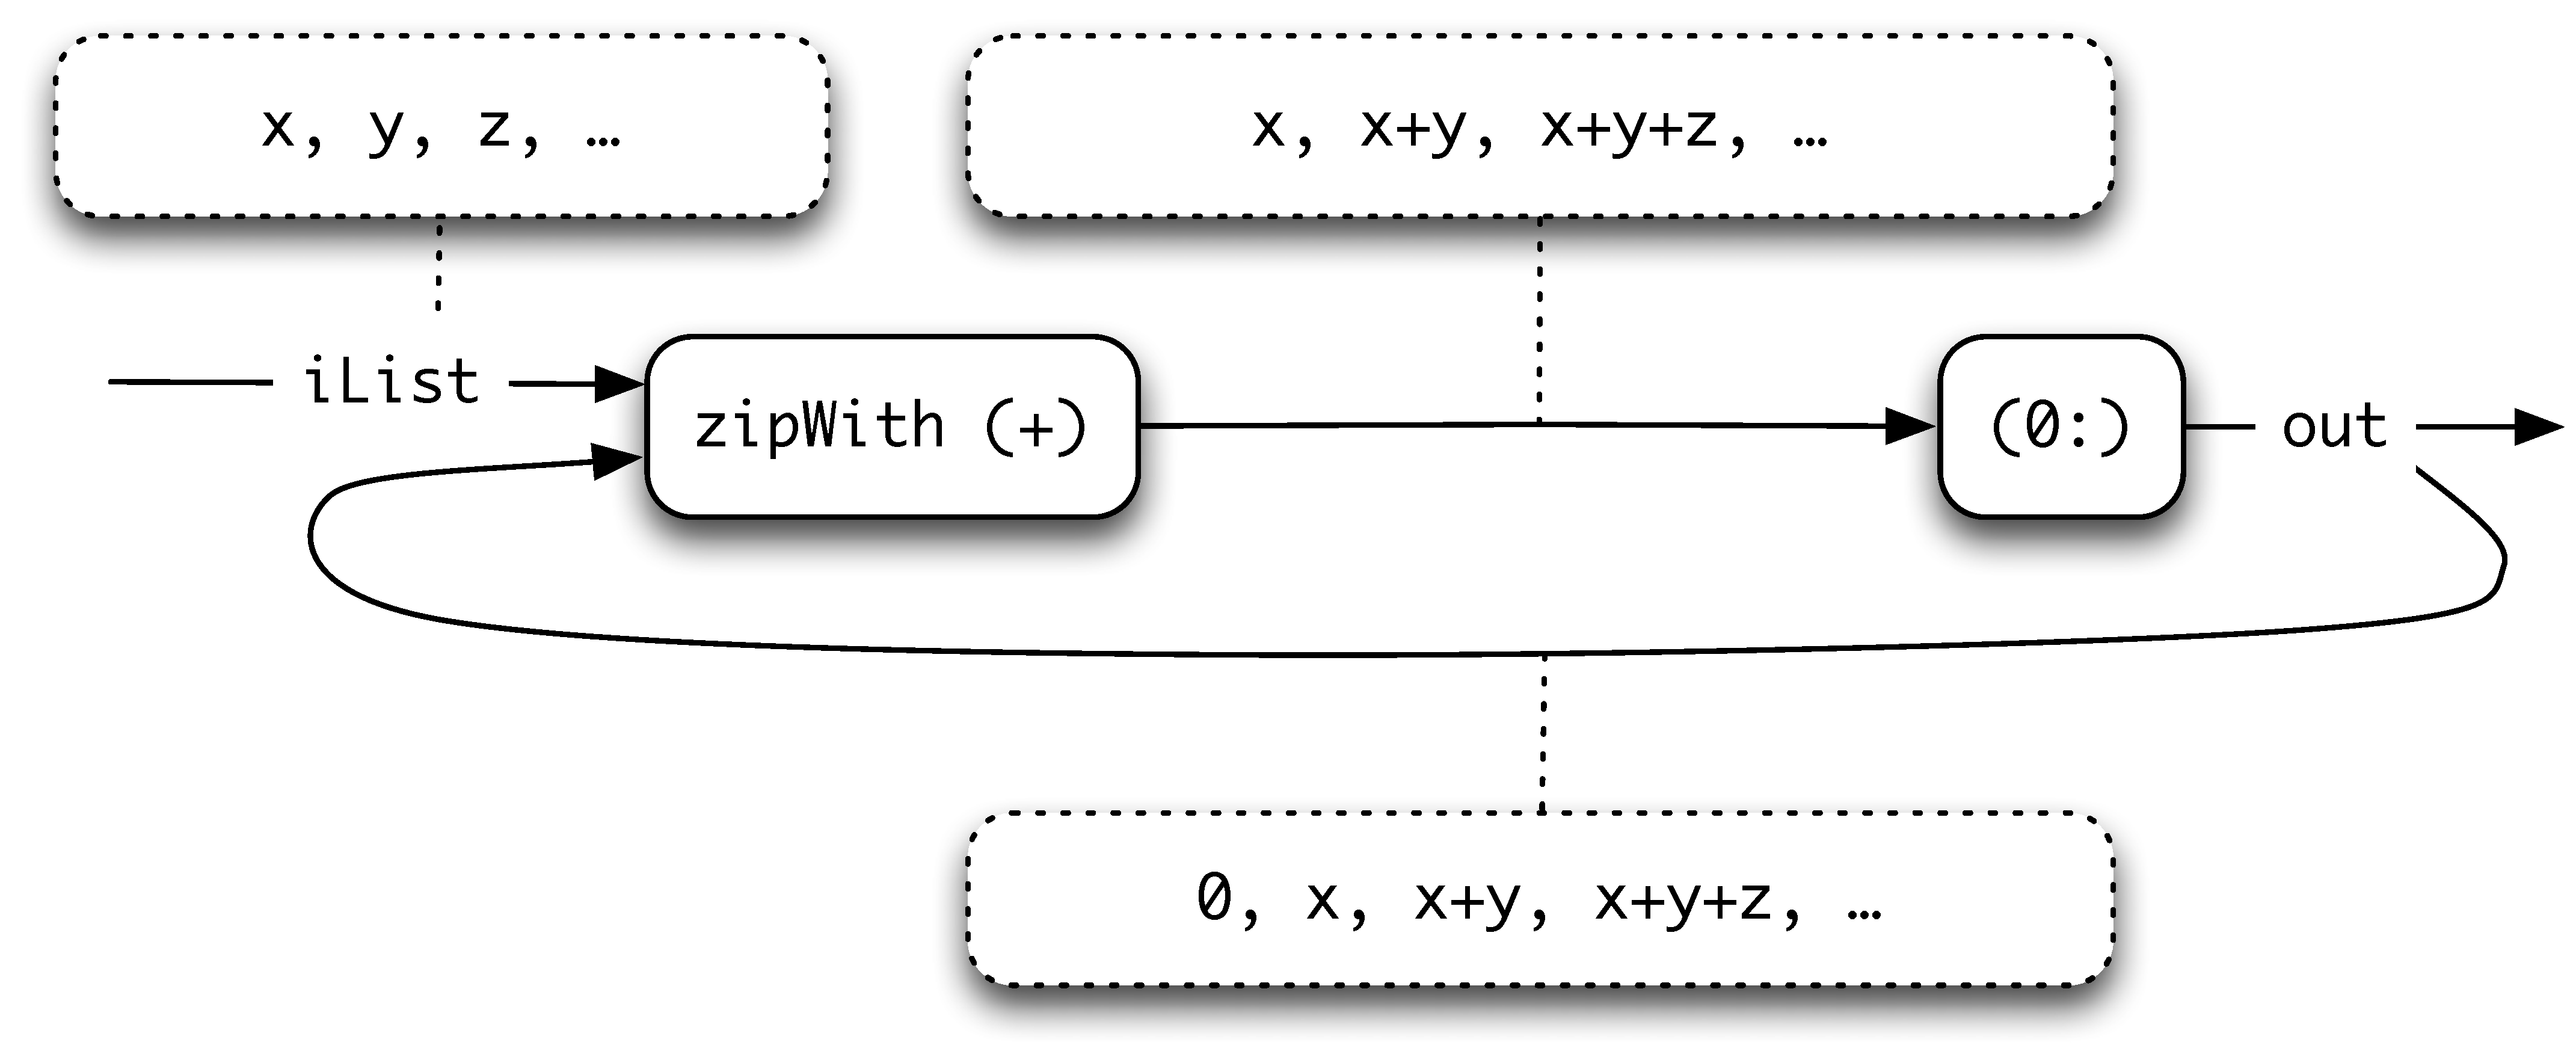
\includegraphics[width=5in]{Pictures/Processes3.pdf}
\end{center}
\caption{A process to compute the running sums of a list.}
\label{sumStream}
\end{figure}

The first value in the output \texttt{out} is \texttt{0}, and we get  the remaining values 
 by adding the next value in \texttt{iList} to the previous sum, appearing in
the list \texttt{out}.
This is translated into Haskell as follows. The output of the function on 
input \texttt{iList} is \texttt{out}. This is itself got by adding \texttt{0} to the
front of the output from the \texttt{zipWith (+)}, which itself has inputs 
\texttt{iList} and \texttt{out}. In other words,
\begin{alltt} 
listSums :: [Integer] -> [Integer]

listSums iList = out
                 where
                 out = 0 : zipWith (+) iList out
\end{alltt} 
where we recall that \texttt{zipWith} is defined by\index{zipWith@\texttt{zipWith}}
\begin{alltt}
zipWith f (x:xs) (y:ys) = f x y : zipWith f xs ys
zipWith f _     _       = []
\end{alltt}
and the operator section \texttt{(0:)} puts a zero on the front of a list. 
We give a calculation of an example now.
\begin{alltt}\minx{listSums}
listSums [1 ..\ ]
\step out
\step 0 : zipWith (+) [1 ..\ ] out
\step 0 : zipWith (+) [1 ..\ ] (0:...) \hfill(1)
\step 0 : 1+0 : zipWith (+) [2 ..\ ] (1+0:...)\hfill(2)
\step 0 : 1 : 2+1 : zipWith (+) [3 ..\ ] (2+1:...)  \step ...
\end{alltt} 
In making this calculation, we replace the occurrence of \texttt{out} in line
\texttt{(1)} with the incomplete list \texttt{(0:...)}. In a similar way, we
replace the tail of \texttt{out} by \texttt{(1+0:...)} in line \texttt{(2)}.

The definition of \texttt{listSums} is an example of the general function \texttt{scanl'},
which combines values using the function \texttt{f}, and whose first output is
\texttt{st}.
\begin{alltt}
scanl' :: (a -> b -> b) -> b -> [a] -> [b]\index{scanl@\texttt{scanl\symbol{39}}}
scanl' f st iList
  = out 
    where
    out = st : zipWith f iList out
\end{alltt}
The function \texttt{listSums} is given by \texttt{scanl' (+) 0}, and a function which
keeps a running sort of the initial parts of list is 
\texttt{sorts = scanl' ins []}, where \texttt{ins} inserts an element in the
appropriate place in a sorted list. The list of factorial values, 
\texttt{\index{factorial}
[1,1,2,6,...]} is given by \texttt{scanl' (*) 1 [1 ..\ ]}, and taking this as a
model, any primitive recursive function \index{primitive recursion}
can be described in a similar way.

The definition we give here is a minor variant of
the standard function \texttt{scanl},\minx{scanl}
but we choose to give the definition here because of its close
correspondence to the process networks for running sums given in Figure
\ref{sumStream}.

\begin{exercises}

\item
Give a definition of the list \texttt{[ 2\^{}n | n <- [0 ..\ ] ]} using a process
network based on \texttt{scanl'}. (Hint: you can take the example of factorial as a
guide.)

\item
How would you select certain elements of an infinite list? For instance, how
would you keep running sums of the {\em positive\/} numbers in a list of
numbers?

\item
How would you {\em merge\/} two infinite lists, assuming that they are
sorted?
How would you remove duplicates from the list which results? As an example,
how would you merge the lists of powers of \texttt{2} and \texttt{3}?

\item
Give definitions of the lists of Fibonacci numbers 
\texttt{\index{Fibonacci numbers}
[0,1,1,2,3,5,...]} and Hamming numbers \texttt{[1,2,3,4,5,6,8,9,...]} (defined on
page \pageref{HamNos}) using 
\index{Hamming numbers}
networks of processes. For the latter problem, you may find
the merge function of the previous question useful.

\index{design!and infinite lists|)}

\end{exercises}

\section{Case study: simulation}
\index{simulation|(}

We are now in a position to put together the ingredients of the queue
simulation covered in 
\begin{titemize}
\item Section \ref{algDesign}, where we designed the algebraic types
\texttt{Inmess} and \texttt{Outmess},
\item Section \ref{simEx}, where the abstract types \texttt{QueueState} and 
\texttt{ServerState} were introduced, and in 
\item Section \ref{infLists}, where we showed how to generate an infinite list
of pseudo-random waiting times chosen according to 
a distribution over the times \texttt{1} to \texttt{6}.
\end{titemize}
As we said in Section \ref{algDesign}, our top-level simulation will be a
function from a series of input messages to a series of output messages, so
\begin{alltt}
doSimulation :: ServerState -> [Inmess] -> [Outmess]
\end{alltt}
where the first parameter is the state of the server at the start of the
simulation. In Section \ref{simEx} we presented the function performing
one step of the simulation,
\begin{alltt}
simulationStep :: ServerState -> 
                  Inmess -> 
                  (ServerState, [Outmess])
\end{alltt}
which takes the current server state, and the input message arriving at the
current minute and returns the state after one minute's  processing, paired
with the list of the output messages produced by the queues that minute (potentially
every queue could release a customer at the same instant, just as no
customers might be released.)

The output of the simulation will be given by the output messages generated
in the first minute, and after those the results of a new simulation beginning
with the updated state:
\begin{alltt}
doSimulation servSt (im:messes)
  = outmesses ++ doSimulation servStNext messes
    where
    (servStNext , outmesses) = simulationStep servSt im
\end{alltt}
How do we generate an input sequence? From Section \ref{infLists} we have the 
sequence of times given by 
\begin{alltt}
randomTimes \minx{randomTimes}
  = map (makeFunction dist . fromIntegral) (randomSequence seed)
  \step [2,5,1,4,3,1,2,5,...
\end{alltt}
We are to have arrivals of one person per minute, so the input messages we
generate are
\begin{alltt}
simulationInput 
  = zipWith Yes [1 ..\ ] randomTimes \minx{simulationInput}
  \step [ Yes 1 2 , Yes 2 5 , Yes 3 1 , Yes 4 4 , Yes 5 3 ,...
\end{alltt}
What are the outputs produced when we run the simulation on this input with
four queues, by setting the constant \texttt{numQueues} to \texttt{4}? The output
begins
\begin{alltt}
doSimulation serverStart simulationInput
\step [Discharge 1 0 2, Discharge 3 0 1, Discharge 6 0 1, 
     Discharge 2 0 5, Discharge 5 0 3, Discharge 4 0 4,
     Discharge 7 2 2,...
\end{alltt}
The first six inputs are processed without delay, but the seventh requires a
waiting time of \texttt{2} before being served. 

The infinite number of arrivals
represented by \texttt{simulationInput} will obviously generate a corresponding
infinite number of output messages. We can make a finite approximation by
giving the input
\begin{alltt}
simulationInput2 = take 50 simulationInput ++ noes
noes = No : noes
\end{alltt}
where after one arrival in each of the first 50 minutes, no further
people arrive. Fifty output messages will be generated, and we define this
list of outputs thus:
\begin{alltt}
take 50 (doSimulation serverStart simulationInput2)
\end{alltt}

\subsection*{Experimenting}
\index{simulation!experimenting}

We now have the facilities to begin experimenting with different data, such
as the distribution and the number of queues. The total waiting time for a
(finite) sequence of \texttt{Outmess} is given by
\begin{alltt}
totalWait :: [Outmess] -> Int
totalWait = sum . map waitTime
            where
            waitTime (Discharge _ w _) = w
\end{alltt}
For \texttt{simulationInput2} the total waiting time is \texttt{29}, going up to
\texttt{287} with three queues and down to zero with five. We leave it to the
reader to experiment with the \textbf{round robin} simulation outlined in the
exercises of Section \ref{simEx}.

A more substantial project is to model a set-up with a single queue feeding a
number of bank clerks -- one way to do this is to extend the 
\texttt{serverState} with an extra queue which feeds into the individual queues: an
element leaves the feeder queue when one of the small queues is empty. This
should avoid the unnecessary waiting time we face when making the wrong
choice of queue, and the simulation shows that waiting times are reduced by
this strategy, though by less than we might expect if service times are short.

\index{simulation|)}
\index{lists!infinite|)}



\section{Proof revisited}
\label{lazyProof}

After summarizing the effect that lazy evaluation has on the types of
Haskell, we examine the consequences for reasoning about programs. Taking lists
as a representative example, we look at how we can prove properties of infinite
lists, and of all lists, rather than simply the set of finite
lists, which was the scope of the proofs we looked at in Chapters
\ref{reasoningProgs}, \ref{gen2} and \ref{algTypes}.

This section cannot give complete coverage of the issues of verification; we
conclude with pointers to further reading.

\subsection*{Undefinedness}
\index{undefinedness}

In nearly every programming language, it is possible to write a program which
fails to terminate, and Haskell is no exception. We call the value of such
programs the \textbf{undefined} value, as it gives no result to a computation.

The simplest expression which gives an undefined result is 
\begin{alltt}
undef :: a\minx{undef}
undef = undef\hfill(undef.1)
\end{alltt}
which gives a non-terminating or
undefined value of every type, but of course we can write an
undefined program without intending to, as in
\begin{alltt}
fak n = (n+1) * fak n
\end{alltt}
where we have confused the use of \texttt{n} and \texttt{n+1} in
attempting to define the
factorial function. The value of \texttt{fak n} will be the same as \texttt{undef}, as they
are both non-terminating.

We should remark that we
are using the term `undefined' in two different ways here. The \textbf{name}
\index{name}
\index{value!undefined}
\texttt{undef} is given a definition by \texttt{(undef.1)}; the \textbf{value} that the
definition gives it is the undefined value, which represents the result of a
calculation or evaluation which fails to terminate (and therefore fails to
define a result).

The existence of these undefined values has an effect on the type of lists.
What if we define, for example, the list
\begin{alltt}
list1 = 2:3:undef
\end{alltt}
The list has a well-defined head, \texttt{2}, and tail \texttt{3:undef}. Similarly,
the tail has a head, \texttt{3}, but its tail is undefined. The type \texttt{[Integer]}
therefore contains \textbf{partial} lists \index{lists!partial}
like \texttt{list1}, built from the
undefined list, \texttt{undef}, parts of which are defined and parts of which are
not.

Of course, there are also undefined
integers, so we also include in \texttt{[Integer]} lists like
\begin{alltt}
list2 = undef:[2,3]
list3 = undef:4:undef
\end{alltt}
which contain undefined values, and might also be partial. Note that in 
\texttt{list3} the first occurrence of \texttt{undef} is at type \texttt{Integer} while the
second is at type \texttt{[Integer]}.

What happens when a function is applied to \texttt{undef}? We use the rules for
calculation we have seen already, so that the \texttt{const} function of the 
standard prelude satisfies
\begin{alltt}
const 17 undef \step 17
\end{alltt}
If the function applied to \texttt{undef} has to pattern match, then the result of
the function will be \texttt{undef}, since the pattern match has to look at the
structure of \texttt{undef}, which will never terminate. For instance, for the
functions used in Chapter \ref{reasoningProgs},
\begin{alltt}
sum undef       \step undef \hfill (sum.u)
doubleAll undef \step undef \hfill (doubleAll.u)
\end{alltt}
In writing proofs earlier in the book we were careful to state that in some
cases the results hold only for \textbf{defined} values. \index{value!defined}

An integer is defined \index{numbers!defined}
if it is not equal to \texttt{undef}; a list is defined \index{lists!defined}
if it
is a finite list of defined values; using this as a model it is not
difficult to give a definition of the defined values of any algebraic type. 
 
A
finite list as we have defined it may contain undefined values. Note that in
some earlier proofs we stipulated that the results hold only for (finite)
lists of defined values, that is for defined lists.



\subsection*{List induction revisited}

As we said above, since there is an undefined list, \texttt{undef}, in each list
type, lists can be built up from this; there will therefore be two base
cases in the induction principle.

\subsubsection*{Proof by structural induction: fp-lists} 
\index{structural induction}

To prove the property \texttt{P(xs)} for all finite or partial lists
(\textbf{fp-lists}) \texttt{xs} we have to do three things:
\index{fp-list}
\index{lists!finite/partial}

\medskip
\noindent
\begin{mytable}
\bf Base cases & Prove \texttt{P([])} and \texttt{P(undef)}. \\
\bf Induction step & Prove \texttt{P(x:xs)} assuming that \texttt{P(xs)} holds
already.
\end{mytable}

\medskip
\noindent
Among the results we proved by structural induction in Chapter \ref{reasoningProgs}
were the equations
\begin{alltt}
sum (doubleAll xs) = 2 * sum xs \hfill (sum-double)\minx{sum}\minx{doubleAll}
xs ++ (ys ++ zs)   = (xs ++ ys) ++ zs\hfill (assoc++)\minx{++}
reverse (xs ++ ys) = reverse ys ++ reverse xs\hfill (reverse++)\minx{reverse}
\end{alltt}
for all \textbf{finite} lists \texttt{xs}, \texttt{ys} and \texttt{zs}. For these results to
hold for all fp-lists, we need to show that
\begin{alltt}
sum (doubleAll undef) = 2 * sum undef \hfill (sum-double.u)
undef ++ (ys ++ zs)   = (undef ++ ys) ++ zs\hfill (assoc++.u)
reverse (undef ++ ys) = reverse ys ++ reverse undef\hfill (reverse++.u)
\end{alltt}
as well as being sure that the induction step is valid for all fp-lists.
Now, by \texttt{(sum.u)} and \texttt{(doubleAll.u)} the equation \texttt{(sum-double.u)} 
holds, and so \texttt{(sum-double)}
holds for all fp-lists. In a similar way, we can show \texttt{(assoc++.u)}.
More interesting is \texttt{(reverse++.u)}. Recall the definition of \texttt{reverse}:
\begin{alltt}
reverse []    = []
reverse (x:xs) = reverse xs ++ [x] 
\end{alltt}
It is clear from this that since there is a pattern match on the
parameter, \texttt{undef} as the first parameter will give an \texttt{undef}
result, so
\begin{alltt}
reverse undef = undef
\end{alltt}
Taking a defined list, like \texttt{[2,3]} for \texttt{ys} in \texttt{(reverse++.u)}
gives
\begin{alltt}
reverse (undef ++ [2,3])
  = reverse undef
  = undef

reverse [2,3] ++ reverse undef
  = [3,2] ++ undef
\end{alltt}
This is enough to show that \texttt{(reverse++.u)} does not hold, and that we cannot
infer that \texttt{(reverse++)} holds for all fp-lists. Indeed the example above shows
exactly that \texttt{(reverse++)} is not valid.

\subsection*{Infinite lists}
\index{lists!infinite}

Beside the fp-lists, there are \textbf{infinite} members of the list types.
How can we prove properties of infinite lists? A hint is given by our
discussion of printing the results of evaluating an infinite list. In practice
what happens is that we interrupt evaluation by hitting \texttt{Ctrl-C}
after some period of time. We can think of what we see on the screen as an
\textbf{approximation}\index{lists!infinite!approximation to} to the infinite list. 

If what we see are the elements 
\texttt{\subscr{a}{0},\subscr{a}{1},\subscr{a}{2},\ldots,\subscr{a}{n}}, we can think
of the approximation being the list
\begin{alltt}
\subscr{a}{0}:\subscr{a}{1}:\subscr{a}{2}:\ldots:\subscr{a}{n}:undef
\end{alltt}
since we have no information about the list beyond the element 
\texttt{\subscr{a}{n}}.

More formally, we say that the partial lists
\begin{alltt}
undef, \subscr{a}{0}:undef, \subscr{a}{0}:\subscr{a}{1}:undef, \subscr{a}{0}:\subscr{a}{1}:\subscr{a}{2}:undef, \ldots
\end{alltt}
are approximations to the infinite list 
\texttt{[\subscr{a}{0},\subscr{a}{1},\subscr{a}{2},\ldots,\subscr{a}{n},\ldots]}. 

Two lists \texttt{xs} and \texttt{ys} are equal if all their
approximants are equal, that is for all natural numbers \texttt{n},
\texttt{take n xs = take n ys}.
(The \texttt{take} function gives the defined portion of the \texttt{n}th
approximant, and it is enough to compare these parts.) A more usable
version of this principle applies to infinite lists only.

\subsubsection*{Infinite list equality}
\index{equality!infinite lists}
A list \texttt{xs} is infinite if for all natural numbers
\texttt{n}, \texttt{take n xs
\noteq\ take (n+1) xs}.\\
Two infinite lists \texttt{xs} and \texttt{ys} are equal if for all natural
numbers \texttt{n},
\texttt{xs!!n = ys!!n}.

\subsection*{Example}
\subsubsection*{Two factorial lists}

Our example here is inspired by the process-based programs of Section
\ref{whyInfLis}. If \texttt{fac} is the factorial function
\begin{alltt}
fac :: Int -> Int\minx{fac}
fac 0 = 1\hfill (fac.1)
fac m = m * fac (m-1)\hfill (fac.2)
\end{alltt}
one way of defining the infinite list of factorials is
\begin{alltt}\minx{facMap}
facMap = map fac [0 ..\ ]\hfill (facMap.1) 
\end{alltt}
while a process-based solution is
\begin{alltt}\minx{facs}
facs = 1 : zipWith (*) [1 ..\ ] facs\hfill (facs.1)
\end{alltt}
Assuming these lists are infinite (which they clearly are), we have to prove
for all natural numbers \texttt{n} that 
\begin{alltt}
facMap!!n = facs!!n \hfill (facMap.!!)
\end{alltt}
\startpr
In our proof we will assume for all natural numbers \texttt{n} the results
\begin{alltt}
(map f xs)!!n        = f (xs!!n)\hfill (map.!!)
(zipWith g xs ys)!!n = g (xs!!n) (ys!!n)\hfill (zipWith.!!)
\end{alltt}
which we discuss again later in this section.
 
\texttt{(facMap.!!)} is proved by mathematical induction\index{mathematical induction},
that is we prove the result for \texttt{0} outright, and we prove the
result for a positive \texttt{n} assuming the result for \texttt{n-1}.

\subparagraph*{Base}
We start by proving the
result at zero. Examining the left-hand side first,
\begin{alltt}
facMap!!0 
  = (map fac [0 ..\ ])!!0 \hfill {\rm by} (facMap.1)
  = fac ([0 ..\ ]!!0) \hfill {\rm by} (map.!!)
  = fac 0\hfill {\rm by def of} [0 ..\ ],!!
  = 1 \hfill {\rm by} (fac.1)
\end{alltt}
The right-hand side is
\begin{alltt}
facs!!0
  = (1 : zipWith (*) [1 ..\ ] facs)!!0 \hfill {\rm by} (facs.1)
  = 1\hfill {\rm by def of} !!
\end{alltt}
thus establishing the base case. 

\subparagraph*{Induction}
In the induction case we have to prove \texttt{(facMap.!!)}
using the induction hypothesis:
\begin{alltt}
facMap!!(n-1) = facs!!(n-1) \hfill (hyp)
\end{alltt}
The left-hand side of \texttt{(facMap.!!)} is
\begin{alltt}
facMap!!n
  = (map fac [0 ..\ ])!!n \hfill {\rm by} (facMap.1)
  = fac ([0 ..\ ]!!n) \hfill {\rm by} (map.!!)
  = fac n \hfill {\rm by def of} [0 ..\ ],!!
  = n * fac (n-1) \hfill {\rm by} (fac.2)
\end{alltt}
It is not hard to see that we have 
\texttt{facMap !!\ (n-1) = fac (n-1)} by a similar argument to the first three steps here
and so,
\begin{alltt}
  = n * (facMap!!(n-1))
\end{alltt}
The right-hand side of \texttt{(facMap.!!)} is 
\begin{alltt}
facs!!n
  = (1 : zipWith (*) [1 ..\ ] facs)!!n \hfill{\rm by} (facs.1)
  = (zipWith (*) [1 ..\ ] facs)!!(n-1) \hfill {\rm by def of} !!
  = (*) ([1 ..\ ]!!(n-1)) (facs!!(n-1))\hfill {\rm by} (zipWith.!!)
  = ([1 ..\ ]!!(n-1)) * (facs!!(n-1))\hfill {\rm by def of} (*)
  = n * (facs!!(n-1)) \hfill {\rm by def of} [1 ..\ ],!!
  = n * (facMap!!(n-1)) \hfill {\rm by} (hyp)
\end{alltt}
The final step of this proof is given by the induction hypothesis, and
completes the proof of the induction step and the result itself. \blackbox

\subsection*{Proofs for infinite lists}

When are results we prove for all fp-lists valid for all lists? If a
result holds for all fp-lists, then it holds for all {\em approximations\/}
to infinite lists. For some properties it is enough to know the property
for all approximations to know that it will be valid for all infinite lists
as well. In particular, this is true for all {\em equations\/}. This means
that, for example, we can assert that for {\em all\/} lists \texttt{xs},
\begin{alltt}
(map f . map g) xs = map (f.g) xs
\end{alltt}
and therefore by the principle of extensionality for functions,
\index{extensionality principle}
\begin{alltt}
map f . map g = map (f.g)
\end{alltt}
Many other of the equations we proved initially for finite lists can be
extended to proof for the fp-lists, and therefore to all lists. Some
of these are given in the exercises which follow.

\subsection*{Further reading}

The techniques we have given here provide a flavour of how to write
proofs for
infinite lists and infinite data structures in general. We cannot give the
breadth or depth of a full presentation, but refer the reader to 
\citeN{logicandcomp} for
more details. An alternative approach to proving the factorial list
example is given in \citeN{sjtProofFP}, which also gives a survey of proof
in functional programming.



\begin{exercises}

\item
Show that for all fp-lists \texttt{ys} and \texttt{zs},
\begin{alltt}
undef ++ (ys ++ zs)  = (undef ++ ys) ++ zs
\end{alltt}
to infer that \texttt{++} is associative over all lists.

\item
If \texttt{rev xs} is defined to be \texttt{shunt xs []}, as
in Section \ref{genPrf}, show that
\begin{alltt}
rev (rev undef) = undef \hfill (rev-rev.1)
\end{alltt}
In Chapter \ref{reasoningProgs} we proved that 
\begin{alltt}
rev (rev xs) = xs \hfill (rev-rev.2)
\end{alltt}
for all
finite lists \texttt{xs}. 

Why can we not infer from \texttt{(rev-rev.1)} and \texttt{(rev-rev.2)}
that the equation \texttt{rev (rev xs) = xs} holds for all fp-lists \texttt{xs}? 

\item
Prove for all natural numbers \texttt{m}, \texttt{n} and functions 
\texttt{f ::\ Int -> a} that 
\begin{alltt}
(map f [m ..\ ])!!n = f (m+n)
\end{alltt}
[Hint: you will need to choose the right variable for the induction proof.]

\item
Prove that the lists
\begin{alltt}
facMap = map fac [0 ..\ ]
facs = 1 : zipWith (*) [1 ..\ ] facs
\end{alltt}
are infinite.

\item
If we define indexing thus
\begin{alltt}
(x:_)!!0  = x
(_:xs)!!n = xs!!(n-1)
[]!!n     = error "Indexing"
\end{alltt}
show that for all strict functions \texttt{f}, fp-lists \texttt{xs} and natural numbers \texttt{n},
\begin{alltt}
(map f xs)!!n = f (xs!!n)
\end{alltt}
and therefore infer that the result is valid for all lists \texttt{xs}.
State and prove a similar result for \texttt{zipWith}.

\item
Show that the following equations hold between functions.
\begin{alltt}
filter p . map f     = map f . filter (p . f)
filter p . filter q  = filter (q \&\&\& p)
concat . map (map f) = map f . concat      
\end{alltt}
where the operator \texttt{\&\&\&} is defined by
\begin{alltt}
(q \&\&\& p) x = q x \&\& p x
\end{alltt}
\end{exercises}

\begin{summary}
Lazy evaluation of Haskell expressions means that we can write
programs in a different style. A data structure created within a program
execution will only be created on demand, as we saw with the example of
finding the sum of fourth powers. In finding routes through a graph we saw
that we could explore just that part of the graph which is needed to reveal a
path. In these and many more cases the advantage of lazy evaluation is to
give programs whose purpose is clear and whose execution is efficient.

We re-examined the list comprehension notation, which
makes many list processing programs easier to express; we saw this in the
particular examples of route finding and parsing.

A design principle exploited in this chapter involved
the use of lazy lists: if a function can return multiple
results it is possible to represent this as a list; using lazy evaluation, the
multiple results will only be generated one-by-one, as they are required.
Also, we are able to represent `no result' by the empty list, \texttt{[]}. This
`list of successes' method is useful in a variety of contexts.

Exploiting this principle as well as higher-order functions, polymorphism and 
list comprehensions we
gave a library of parsing functions, which we saw applied to the type of
arithmetical expressions, \texttt{Expr}. This showed one of the strengths of
modern functional programming languages, whose constructs are especially well
suited to describing general toolkits of this sort.

Rather than being simply a curiosity, this chapter has shown that we can
exploit infinite lists for a variety of purposes.
\begin{titemize}
\item In giving an {\em infinite\/} list of prime or random numbers we
provide an unlimited resource: we do not have to know how much of the
resource we need while constructing the program; this {\em abstraction\/}
makes programming simpler and clearer.
\item Infinite lists provide a mechanism for process-based programming in
a functional setting.
\end{titemize}

The chapter concluded with a discussion of how proofs could be lifted to the
partial and infinite elements of the list type: criteria were given in both
cases  and we gave examples and counter-examples in illustration.

\end{summary}

%\end{document}
